\documentclass[9pt,twocolumn,twoside]{pnas-new}
% Use the lineno option to display guide line numbers if required.

\templatetype{pnasresearcharticle} % Choose template
% {pnasresearcharticle} = Template for a two-column research article
% {pnasmathematics} %= Template for a one-column mathematics article
% {pnasinvited} %= Template for a PNAS invited submission

% riccardo
\usepackage{siunitx}
\usepackage{physics}
\newcommand{\SNR}{\mathrm{SNR}}

\begin{document}


\title{
%Chemotactic encounters between bacteria and phytoplankton -- outsized payoffs for small phytoplankton cells
Chemotactic encounters between bacteria and phytoplankton -- the stakes are high for encounters with small phytoplankton.
}
% DB: I would consider substituting one instance of "encounter" with a different word. For example, replace the first casee with "interactions".

% Use letters for affiliations, numbers to show equal authorship (if applicable) and to indicate the corresponding author
\author[a]{Riccardo Foffi}
\author[b]{Douglas R. Brumley}
\author[c]{François Peaudecerf}
\author[a]{Roman Stocker}
\author[a,1]{Jonasz S\l{}omka}

\affil[a]{Institute of Environmental Engineering, Department of Civil, Environmental and Geomatic Engineering, ETH Z\"urich, 8093 Z\"urich, Switzerland}
\affil[b]{School of Mathematics and
Statistics, The University of Melbourne, Parkville, Victoria, Australia}
\affil[c]{Univ Rennes, CNRS, IPR (Institut de Physique de Rennes) - UMR 6251, F-35000 Rennes, France}


% Please give the surname of the lead author for the running footer
\leadauthor{Foffi}

% Please add a significance statement to explain the relevance of your work
\significancestatement{
Swimming bacteria search for phytoplankton to exchange metabolites, which control nutrient cycling in the ocean. Chemotaxis can accelerate the search by navigating bacteria along gradients of chemicals exuded by phytoplankton. However, successful navigation requires bacterial detection of noisy gradients, yet the type of noise depends on phytoplankton size. 
%DB: "...of noisy gradients, with the type of noise depending on the size of the phytoplankton targets."
Detection fails when gradients are too flat (large phytoplankton) or too spatially confined (small phytoplankton). We computed an upper bound on chemotaxis's advantage for different phytoplankton size classes and found that chemotaxis offers the largest reductions in search time for small phytoplankton. However, the advantage sensitively relies on bacteria's chemotactic strategy. Chemotactic encounters with small phytoplankton are thus a high-stakes game that may promote a diversity of size-dependent chemotactic strategies.
%Authors must submit a 120-word maximum statement about the significance of their research paper written at a level understandable to an undergraduate educated scientist outside their field of speciality. The primary goal of the significance statement is to explain the relevance of the work in broad context to a broad readership. The significance statement appears in the paper itself and is required for all research papers.}
}
% Please include corresponding author, author contribution and author declaration information
\authorcontributions{Please provide details of author contributions here.}
\authordeclaration{Please declare any competing interests here.}
%\equalauthors{\textsuperscript{1}R.F. and J.S. contributed equally to this work.}
\correspondingauthor{\textsuperscript{1}To whom correspondence should be addressed. E-mail: jonasz.slomka@gmail.com}

% At least three keywords are required at submission. Please provide three to five keywords, separated by the pipe symbol.
\keywords{encounter rates $|$ chemotaxis $|$ bacteria-phytoplankton interactions $|$ microbial ecology}


\begin{abstract}
Chemotaxis, the ability to navigate along chemical gradients, enables motile bacteria to increase encounter rates with symbiotic partners such as phytoplankton cells.
%DB: do we want to start with "symbiosis" as the main pitch? This is a specific type of encounter, but the advantage of chemotaxis is not limited to this situation.
However, it remains unclear how strongly chemotactic encounters depend on the bacterial strategy employed to detect noisy and spatially confined gradients around phytoplankton of different sizes.
%the bacterial strategy to detect noisy and spatially confined gradients controls encounters with different phytoplankton size classes. 
%However, how strongly the bacterial strategy to detect noisy and spatially confined gradients around phytoplankton of different sizes controls encounters remains unclear.
%However, it remains unclear how strongly the ability of bacteria to detect noisy and spatially confined gradients controls encounters with different phytoplankton size classes. 
Here, we compute analytically and numerically an upper bound on the chemotactic index, a dimensionless number that measures the increase in encounter rate with a phytoplankton cell due to chemotaxis over random motility alone. 
%We study how the chemotactic index depends on phytoplankton's size, the concentration and diffusivity of the chemoattractant, and the bacterium's swimming speed, run length, and sensory timescale.
%We find that chemotaxis potentially strongly favors searches for small phytoplankton, owing to the ballistic nature of the encounter for those cells, but the magnitude of the chemotactic index is very sensitive to the concentration and diffusivity of the chemoattractant, and the bacterium's swimming speed, run length, and sensory timescale. 
We find that chemotaxis potentially strongly enhances the efficiency of searches for small phytoplankton, 
% DB: I would ditch the word "potentially" for "can strongly enhance".
owing to the ballistic nature of the encounter for those cells, but the magnitude of the chemotactic index is very sensitive to the bacterial ability to detect spatially confined gradients.
For example, in productive waters, chemotaxis can decrease the search times of bacteria for micron-sized picophytoplankton by more than ten-fold, from days to a few hours. 
%Still, this reduction relies sensitively on the ability of bacteria to detect gradients -- reducing by half the phytoplankton radius or doubling the bacterial swimming speed can render gradients undetectable and erase the benefit of chemotaxis.
Still, this benefit of chemotaxis is easily erased -- reducing by half the phytoplankton radius or doubling the bacterial swimming speed renders gradients undetectable.
For larger phytoplankton (radius $\sim\SI{30}{\micro\meter}$), the decrease in the search time is more moderate, from a month to a week, and depends gently on gradient detection. Thus, engaging chemotaxis in interactions with small phytoplankton is a high-stakes game for bacteria: the potential payoff is large, but it changes abruptly with bacterial ability to sense gradients, a scenario that may promote a diversity of chemotactic strategies.
%Chemotaxis, the ability to sense and navigate along chemical gradients, enables motile bacteria to increase encounters with targets, including nutrient sources and symbiotic partners such as phytoplankton cells, which leak chemoattractants that bacteria use as navigational cues. 
%However, we lack quantitative estimates of the potential increase in chemotaxis-assisted encounters compared to random motility. Here, we use analytical and numerical models to compute an upper bound on the chemotactic index, a dimensionless number that measures the increase in encounter rate with a target due to chemotaxis, over random motility alone. We consider an idealized chemotactic bacterium that always finds a spherical target, provided it successfully detects chemical gradients at some distance away from the target. The detection fails, however, if the gradients are too shallow or too spatially confined. We derive a general equation that predicts how the chemotactic index depends on the target's size, the concentration and diffusivity of the chemoattractant, and the bacterium's swimming speed, run length, and sensory timescale. We find that chemotaxis confers the most prominent advantage for small targets, owing to the ballistic nature of the encounter for those targets. For example, chemotaxis can decrease search times of bacteria for phytoplankton by an order of magnitude for .... The typical search times for picocyanobacteria, the smallest yet most abundant phytoplankton cells in the oceans, can decrease from multiple days to a few hours, provided that bacteria move slower and measure gradients more accurately. 
%%For bacterial interactions with realistic phytoplankton communities, such as those in oligotrophic or productive aquatic environments, chemotaxis can reduce the bacterial search time of the smallest yet most abundant phytoplankton cells by an order of magnitude.
%Such an outsized payoff for micron-sized phytoplankton cells may drive an evolutionary pressure for bacteria to develop chemotactic strategies other than the classic gradient ascend.
\end{abstract}

\dates{This manuscript was compiled on \today}
\doi{\url{www.pnas.org/cgi/doi/10.1073/pnas.XXXXXXXXXX}}


\maketitle
\thispagestyle{firststyle}
\ifthenelse{\boolean{shortarticle}}{\ifthenelse{\boolean{singlecolumn}}{\abscontentformatted}{\abscontent}}{}

%\firstpage[7]{7}
% Use \firstpage to indicate which paragraph and line will start the second page and subsequent formatting. In this example, there are a total of 11 paragraphs on the first page, counting the first level heading as a paragraph. The value {12} represents the number of the paragraph starting the second page. If a paragraph runs over onto the second page, include a bracket with the paragraph line number starting the second page, followed by the paragraph number in curly brackets, e.g. "\firstpage[4]{11}".

% \section*{Introduction}
% general context

%% Introduction
%First paragraph. A sentence or two on what chemotaxis is (cite Berg + some review). A sentence or two on how chemotaxis can facilitate encounters or metabolic exchanges with symbiotic partners (reviews by Seymor and JB, Jackson and Kiorboe paper, JB's paper Nat Microbiol 2023). Sentence on noise sources: ramp sensing (papers by Wingreen, Doug and Francesco). Gap sentence: however, many phytoplankton are small and they may produce spatially confined gradients, beyond flat ones, and it remains unknown how the spatial confinement affects bacteria's ability to detect cells and hence encounter rates and how sensitive is the potential gain in encounters to the ability of bacteria to detect gradients. This is particularly important in combination with the ballistic nature of the encounter with small targets (Slomka et al NJP).

%Chemotaxis is a widespread mechanism in motile microorganisms to detect and navigate chemical gradients. In bacteria, chemotaxis operates by sensing temporal changes in the concentration of chemoattractant compounds and biasing bacterial motion towards regions where attractant concentrations are higher~\cite{macnab1972gradientsensing,brown1974temporal}.

%Based on a molecule counting process, chemotaxis is inherently subject to noise, especially at low attractant concentrations~\cite{berg1977physics,tenwolde2016fundamental}.
%The limits that noise imposes on chemosensing are well characterized for wide, linear concentration ramps, typical of classical laboratory assays~\cite{mora2010limits}, and for intense but short-lived gaussian pulses, comparable to cell lysis events~\cite{hein2016physical,brumley2019bacteria}.
%The importance of noise for chemotaxis can be especially appreciated in oceanic environments, where nutrient concentrations are often extremely low~\cite{lee1975amino} and being able to cut through the noise and increase the probability to encounter a nutrient hotspot or a symbiotic partner can determine life or death for a bacterium~\cite{brumley2020cutting}.

%In the water column, phytoplankton cells generate complex chemical landscapes by leaking dissolved organic compounds which can be strong attractants for bacteria~\cite{thornton2014dissolved,smriga2016chemotaxis,seymour2017zooming}. The ability of bacteria to navigate these gradients and reach proximity with phytoplankton cells can be crucial for establishing symbiotic relationships and favoring metabolic exchanges~\cite{raina2019role,raina2022chemotaxis} which lie at the heart of oceanic carbon cycles~\cite{azam1998microbial}.
%The composition of marine phytoplankton communities can span up to two orders of magnitude in cell size, from $\sim\SI{0.5}{\micro\m}$ to $\sim\SI{100}{\micro\m}$, with the smallest cells being by far the most abundant~\cite{sprules1986plankton,cermeno2008species}. While larger cells may easily produce gradients extending from tens to hundreds of microns, the chemoattractant fields produced by the micron-sized picoplankton may be relatively weak and/or confined to small spatial regions, requiring chemotactic bacteria to tackle the additional problem of spatial resolution, a significantly different scenario from those that have been classically investigated.
%How sensing noise and spatial confinement jointly affect the success of bacterial chemotactic searches across the water column is therefore unclear.

%The composition of marine phytoplankton communities is vastly dominated by small micron-sized cells~\cite{} which may produce gradients of attractants that are relatively weak and confined over small spatial regions, a significantly different scenario from those that have been classically investigated.
%An understanding of how the additional problem of spatial confinement affects the efficiency of noisy chemotactic searches is therefore still lacking, especially 

Chemotaxis, the ability of bacteria to navigate chemical gradients and reach proximity with phytoplankton cells, can be crucial for establishing symbiotic relationships and favoring metabolic exchanges which lie at the heart of oceanic carbon cycles~\cite{azam1998microbial,raina2019role,raina2022chemotaxis}.
In the water column, phytoplankton cells generate complex chemical landscapes by leaking dissolved organic compounds which can be strong attractants for bacteria~\cite{thornton2014dissolved,smriga2016chemotaxis,seymour2017zooming}.
The composition of marine phytoplankton communities, which can span two orders of magnitude in cell size, from $\sim\SI{0.5}{\micro\m}$ to hundreds of microns~\cite{sieburth1978pelagic}, exposes bacteria to gradients on a wide range of scales.

Bacterial chemotaxis operates by sensing temporal changes in the concentration of chemoattractant compounds and biasing bacterial motion towards regions where these chemoattractant concentrations are higher~\cite{macnab1972gradientsensing,brown1974temporal}. Based on a molecule counting process, chemotaxis is inherently subject to noise \cite{berg1977physics,tenwolde2016fundamental}, especially at the low attractant concentrations typical of oceanic environments~\cite{lee1975amino}.
The limits that noise imposes on chemosensing are well characterized for wide concentration ramps~\cite{mora2010limits}, typical of laboratory assays and comparable to the gradients generated by large phytoplankton cells, and for intense but short-lived gaussian pulses, mimicking cell lysis events~\cite{hein2016physical,brumley2019bacteria}.
By contrast, our understanding of chemotaxis towards small cells, which may generate gradients tightly confined in space, is rather limited, despite the smallest phytoplankters being by far the most abundant~\cite{sprules1986plankton,cermeno2008species}. Moreover, while it is qualitatively well understood that chemotaxis can favor bacteria-phytoplankton interactions, it is quantitatively unclear how much interaction rates can increase across the size spectrum.
% DB: I think it could be worth citing here the 2023 Nature Microbiology paper (https://www.nature.com/articles/s41564-023-01327-9) which demonstrates that chemotaxis does play a role interactions at this scale, enhancing nutrient exchange between micron-sized cells.
% DB: We have a paper in press at Trends in Microbiology "Swimming towards each other: The role of chemotaxis in bacterial interactions" which is also highly relevant to this discussion. It should come out in the next week or so, and I'll be sure to send you a copy.

Here we investigate, through the lens of encounter rates, how chemotaxis can increase interaction rates between bacteria and phytoplankton cells~\cite{slomka2023encounter}. Combining constraints on the detection of noisy and spatially confined gradients with the size-dependent nature of random encounters, we obtain an upper bound on the possible increase in encounter rates resulting from the use of chemotaxis, with respect to purely random searches. Our results, also supported by a numerical model of an ideal sensor, show that chemotaxis towards large phytoplankton cells offers easily accessible but modest reductions in search times; search times for the small picophytoplankton can instead decrease drastically although the risk of failure is high. We hypothesize that such low-risk/low-gain performance for large targets and high-risk/high-gain for small targets may promote size-sensitive chemotactic strategies.


\begin{figure*}
    \centering
    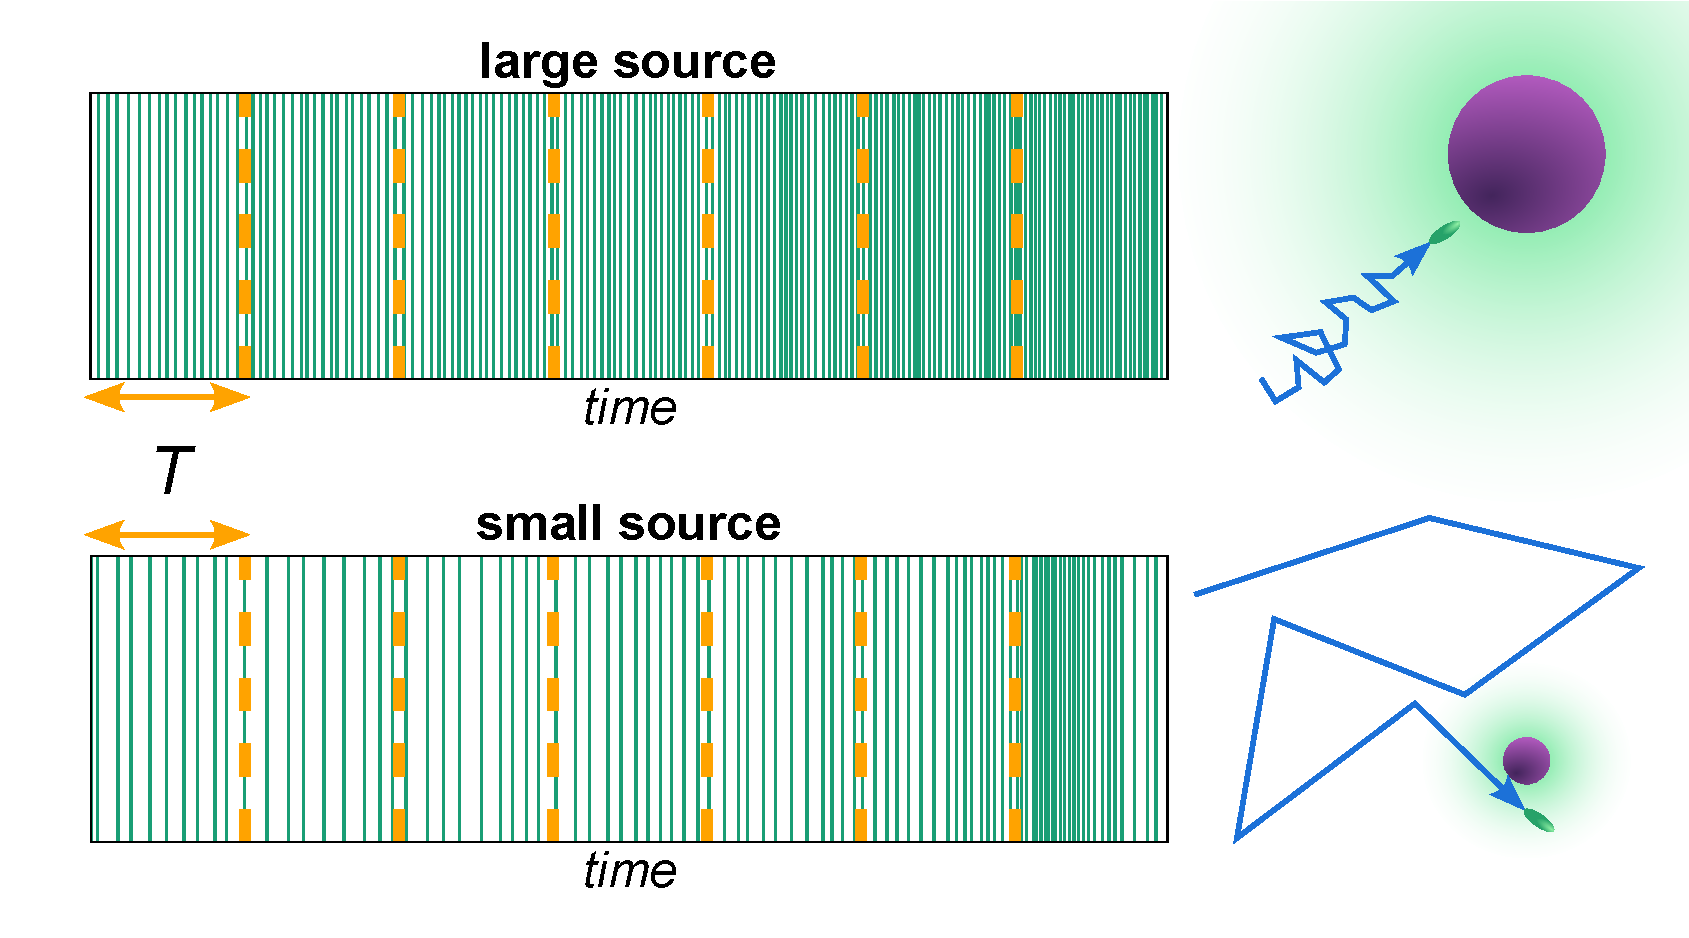
\includegraphics[width=17.8cm]{fig1_new.pdf}
    \caption{
        \textbf{
        Detecting chemical gradients to increase encounter rates with phytoplankton through chemotaxis is a size-dependent challenge for bacteria.
        }
        To estimate the local concentration gradient, the bacterial chemosensory machinery integrates absorption sequences of chemoattractant molecules over a characteristic sensory timescale $T$.
        %The bacterial chemosensory machinery integrates these sequences over a characteristic sensory timescale $T$ to produce an estimate of the local concentration gradient.
        The phytoplankton size determines the lengthscale over which the gradients extend, leading to absorption sequences with well-distinguished features for small and large sources.
        The limiting factors for the detection of these sources are therefore of different nature: sensing noise for large sources arising from molecular fluctuations and dynamic noise for small sources resulting from bacterial motion and limited temporal resolution.
        % DB: Could it be worth mentioning a little more here about the nature of the gradients? i.e. how the time-series is produced.
    }
    \label{fig:setup}
\end{figure*}

Phytoplankton cells of different sizes generate chemical gradients of varying steepness and spatial extent, posing fundamentally different gradient detection challenges for bacteria (Fig.~\ref{fig:setup}; see also discussion in SI).
Bacteria experience concentration fields in the form of temporal sequences of molecular adsorption events, which are integrated over a sensory timescale $T$ to form an estimate of the local concentration gradient~\cite{berg1977physics}. When moving in the chemoattractant field generated by a large phytoplankton cell, which may be characterized by wide spatial extent and a shallow gradient, a bacterium will experience a large baseline adsorption rate with only a gradual increase over subsequent sensory windows. Detection can fail if the gradient is too shallow, and the concentration increase is masked by fluctuations in the molecular adsorption events, a scenario which has been modeled in detail before~\cite{mora2010limits}.
% DB: I think we need to elaborate a bit more on why detection of large gradients can fail. The immediate response would be that far-reaching gradients are likely to be stronger, which compensates for this noise. 
By contrast, in the case of a small phytoplankton cell, whose concentration fields are likely to be weaker and tightly localized in space, the signal will mostly be indistinguishable from the background, until, at very close distance from the phytoplankter, the bacterium will experience a sudden burst in adsorption events localized within a short time interval.
Here the limiting factor is not the inherent noise arising from molecular fluctuations, but the dynamic noise resulting from bacterial motion, which limits the ability of the bacteria to properly resolve a signal appearing over timescales comparable or smaller to the sensory timescale $T$: the limited temporal resolution of the measurements may lead to aliasing effects~\cite{}, preventing an accurate reconstruction of the gradient.
% DB: Here you could cite something like the volcano effect.
Spatially confined sources have received less attention after Jackson proposed that chemotaxis towards cells smaller than $3\sim\SI{4}{\micro\m}$ would not be possible~\cite{jackson1987simulating}; recently, however, it was shown that marine bacterium \emph{Marinobacter adhaerens} can use chemotaxis to increase nutrient uptake from the picocyanobacterium \emph{Synechococcus}~\cite{raina2023chemotaxis}, highlighting how chemotaxis might be relevant even at the smallest scales.
% DB: It could be worth also citing Richard's Synechococcus paper here: https://www.biorxiv.org/content/10.1101/2023.10.24.563588v1.
To study how the phytoplankton size and the associated sensing limitations affect chemotaxis performance, we next outline how to compute an upper bound on the chemotactic index, a dimensionless number that measures the increase in encounter rate with a phytoplankton cell due to chemotaxis over random motility alone.
%Using idealized models of bacterial and phytoplankton behavior, we design a system where the bacterium randomly explores the environment and employs chemotaxis to guide its motion towards the target phytoplankton cell which is leaking chemoattractant (Fig.~\ref{fig:setup}).
%A bacterium is a spherical particle of radius $a = \SI{0.5}{\micro\m}$ (assumed fixed throughout the article), which, in the absence of chemoattractant fields, performs a random walk with speed $U$ and correlation length $\lambda$.
%A phytoplankton cell is a spherical particle of radius $R$ which, exuding organic compounds through its cell wall at constant rate, generates a stationary spatial field of chemoattractant of the form



\begin{figure*}
    \centering
    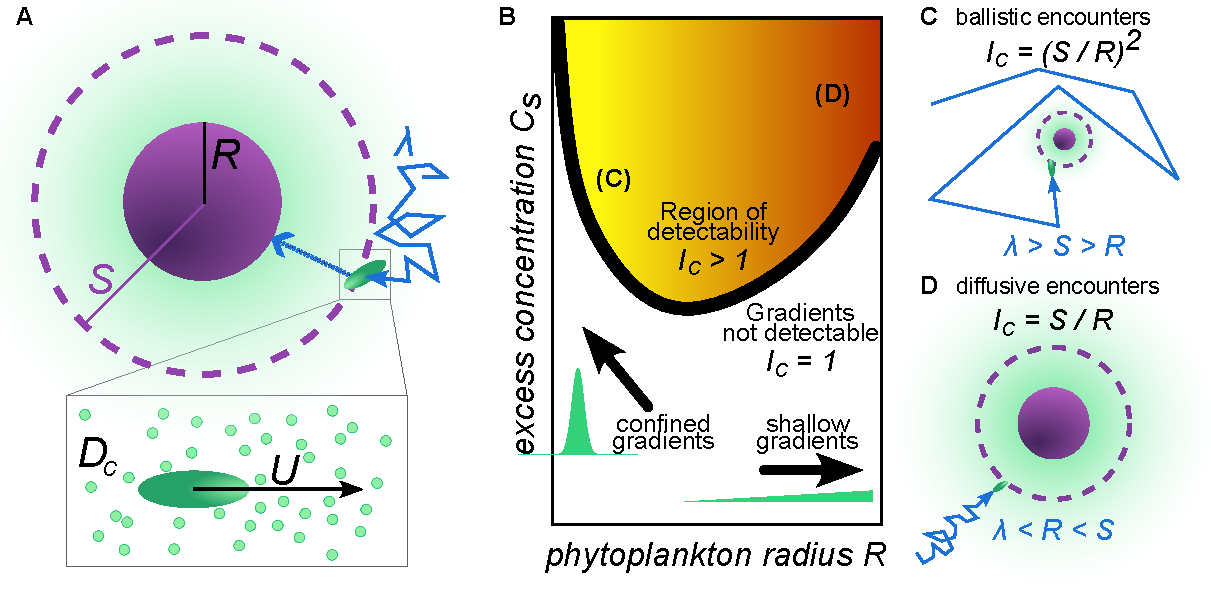
\includegraphics[width=17.8cm]{fig2_new.pdf}
    \caption{
        \textbf{
        %Gradient's steepness and spatial extent determine the ballistic or diffusive nature of bacterial encounters with the sensing region.
        Chemotactic encounters are limited by the gradients' steepness and spatial extent, and ballistic or diffusive encounters with the sensing horizon.
        %Source size and gradient lengthscale determine differences in chemotactic performance.}
        %Bacteria can detect gradients if they are sufficiently steep and spatially extended.}
        }
        (A) A phytoplankton cell of radius $R$ produces a stationary diffusive field of a chemoattractant, $C(r) = C_0 + C_s R/r$ (represented by the green halo).
        Far away from the cell, bacteria cannot sense the chemoattractant and thus swim in random walks, with correlation length $\lambda$.
        %Upon reaching a distance $S$ (the 'sensory distance'), a perfect chemotaxer is able to encounter the cell with 100\% probability.
        The ``sensory distance'' $S$ is the distance from the phytoplankton cell at which a perfect chemotaxer would be able to detect the gradient and encounter its target with a 100\% probability.
        (Inset) Chemosensing is a molecule-counting process based on encounters between the bacterium and individual chemoattractant molecules.
        Attractant molecules reach the bacterium via diffusion (diffusivity $D_c$) while the bacterium swims at speed $U$ through the chemoattractant field.
        (B) Schematic depiction of the performance landscape for chemotactic searches.
        The source size $R$ and the chemoattractant concentration $C_s$ determine whether gradients can be successfully detected or not.
        The thick black line defines the boundary of detection, separating the regions where gradient detection is or is not possible.
        Below the boundary, two conditions limit an organism's ability to perform chemotaxis: gradients are either too spatially confined or too shallow. In this region, chemotaxis provides no benefit over random motility.
        % DB: Can you also specify what parameters "above" and "below" correspond to, so that it's not just linked to the actual plot?
        Above the boundary gradients can be detected, and the increase in encounters compared to random motility, measured by the chemotactic index $I_c$, is determined by the relationship between bacterial correlation length $\lambda$, source size $R$ and sensory radius $S$.
        The size dependence of random encounters identifies two subregions within the region of detectability (yellow-red shading), in which the chemotactic index displays two distinct behaviors.
        Small sources (C) lead to ballistic encounters for which the chemotactic index scales quadratically with the sensory radius $S$, whereas for large sources (D) the chemotactic index scales only linearly with $S$ due to the diffusive nature of encounters.
        % DB: You mention the yellow-red shading. This appears to account for the difference between ballistic and diffusive encounters. It this just a qualitative shading or a heatmap of some kind?
    }
    \label{fig:sensing}
\end{figure*}



%The limits of bacterial gradient detection are regulated by the gradients' steepness and spatial extent.
We compute an upper bound on the chemotactic index by considering a perfect chemotactic bacterium limited only by random encounters with a sensing horizon - a distance inside which the bacterium detects gradients and flawlessly navigates towards the phytoplankton (Fig.~\ref{fig:sensing}).
% DB: When you say "flawless", I think it is worth explicitly mentioning that you mean ballistic motion (even though it is shown graphically in the figure).
We represent a phytoplankton cell as a sphere of radius $R$ which can exude chemoattractants to generate a diffusive concentration field (see SI for derivation and discussion of other concentration fields)
\begin{equation}\label{chemoattractant_field}
    C(r) = C_0 + C_s \dfrac{R}{r}
\end{equation}
where $C_0$ is the background concentration of the compound far away from the phytoplankton cell, $C_s$ is the excess concentration of the compound at the phytoplankton cell surface, and $r$ is the radial distance from the center of the phytoplankton cell ($r\geq R$).
In the absence of chemoattractants, a bacterium performs a random walk with speed $U$ and correlation length $\lambda$. When chemoattractant gradients are present, the bacterium can bias its motion in the direction of the positive gradient, increasing its chances of encountering a leaking phytoplankton cell. We find an upper bound to the encounter-enhancing effect of chemotaxis by considering the bacterium to be a ``perfect chemotaxer'': there exists a ``sensory horizon'', $S$, around the phytoplankton cell where the bacterium can reliably detect the gradient and exploit it to, eventually, yield an encounter with 100\% probability; outside the sensory horizon no chemotactic behavior is manifested (Fig.~\ref{fig:sensing}A).
The problem of chemotactic encounters with the chemoattractant source is therefore reduced to the problem of identifying the sensory horizon.
% DB: Here you have defined a threshold value, which sets up a 'step function' in the chemotactic behaviour. If space permits, it would be nice to explain why this is useful/valid comparison with a real cell, which would have a gradual reponse as a function of r.

The extent of the sensory horizon is defined by the bacterial ability to detect a signal (i.e., a positive gradient) at a given location, as determined by the signal-to-noise ratio.
%; mathematically, this condition can be implemented by requiring the signal-to-noise ratio ($\SNR$) to be higher than some threshold value ($q$). Given expressions for the signal and the noise (both inherent and dynamic), the sensory horizon is therefore the maximal distance from the phytoplankton cell at which $\SNR > q$.
Chemotaxis operates through the adsorption of attractant molecules, which reach the bacterial cell surface with diffusivity $D_c$ (Fig.~\ref{fig:sensing}A inset)~\cite{berg1977physics}; the swimming speed, $U$, determines the temporal gradient experienced by the bacterium, $U\nabla C$~\cite{berg1977physics,hein2016physical}.
In gradients with wide spatial extent, the inherent noise in the gradient measurements, arising from fluctuations in molecular adsorptions, was derived by Mora \& Wingreen~\cite{mora2010limits} as $\sigma_0 = \sqrt{3C/(\pi a D_c T^3)}$; at any given location in space (assuming the bacterium is heading straight towards the phytoplankton cell) the signal-to-noise ratio ($\SNR$) is then given by
\begin{equation}\label{eq:snr_mora}
    \SNR = \dfrac{|U\nabla C|}{\sqrt{3C/(\pi a D_c T^3)}}.
\end{equation}
The $\SNR$ quantifies the likelihood to measure a positive gradient: 
% DB: or ..."related to the likelihood that a positive gradient can be resolved". Need to be a little careful with the language so that it doesn't imply it is a probability.
when $\SNR$ is high, bacteria have a high probability to detect positive gradients; when it is low, gradients are masked by fluctuations.
\eqref{eq:snr_mora} assumes that the concentration field does not vary significantly on times shorter than the sensory timescale $T$, ignoring the contribution of dynamic noise to gradient sensing. We phenomenologically include the dynamic noise contribution by replacing the signal $U\nabla C$ with a discrete approximation $U\nabla_T C$ which takes into account the effect of motion during the finite sensory timescale (detailed discussion in SI).
Further, following Brumley \textit{et al.}~\cite{brumley2019bacteria}, we introduce a chemotactic precision factor $\Pi$ in front of the Mora-Wingreen noise $\sigma = \Pi\sigma_0$, which in marine bacterium \textit{Vibrio anguillarum} was estimated as $\Pi\approx6$.
%The swimming speed $U$ determines the temporal gradient experienced by the bacterium, $U\nabla_T C$, but does not directly affect molecular adsorption rates~\cite{berg1977physics,hein2016physical}; the $\nabla_T$ symbol represents a discrete approximation to the gradient $\nabla$, which takes into account the finite sensory timescale associated to bacterial measurements, and hence implicitly includes the contribution of the dynamic noise (detailed discussion in SI). The gradient measurement process is subject to poissonian fluctuations in the adsorption of chemoattractant molecules which pose a fundamental limit on its precision; the theoretical lower limit on the noies resulting from these fluctuations was estimated by Mora \& Wingreen as $\sigma = \sqrt{3C/(\pi a D_c T^3)}$~\cite{mora2010limits}, and later Brumley \textit{et al.} showed that marine bacteria operate close to (but not exactly at) this theoretical limit and the noise could be well-described by simply including a prefactor $\Pi\approx6$~\cite{brumley2019bacteria}.
%The inherent noise associated to this gradient measurement can be expressed as $\approx 6\sqrt{3C/(\pi a D_c T^3)}$~\cite{mora2010limits,brumley2019bacteria}.
%The relationship between the ``real'' local gradient, the dynamic noise and the inherent noise, which will in general involve both bacterial and environmental parameters, determines the likelihood of the bacteria being able to detect a positive gradient at any given location in space; this relationship can be synthesized into a signal-to-noise ratio ($\SNR$), leading to a natural definition for the sensory horizon $S$ as the farthest distance from the source at which the $\SNR$ overcomes a certain threshold. Mathematically, the sensory horizon $S$ is then the solution to the equation
We then define the sensory horizon $S$ as the farthest distance from the phytoplankton cell at which the $\SNR$ overcomes a threshold $q$; mathematically, $S$ is therefore the solution to the equation
\begin{equation}
    \SNR = \dfrac{|U\nabla_T C_{(S)}|}{\Pi\sigma_{(S)}} =
    \dfrac{|U\nabla_T C_{(S)}|}{6\sqrt{3C_{(S)}/(\pi a D_c T^3)}} = q.
\end{equation}
A reasonable choice is $q=1$, which equates to defining $S$ as the distance where bacteria can detect a positive gradient with a probability $\approx 84\%$ (SI).
%We thus define the sensory horizon $S$ as the distance from the source at which the signal-to-noise ratio (SNR) overcomes a threshold value; in other words, $S$ is the solution to the equation
%\begin{equation}
%    \mathrm{SNR} = \dfrac{U\nabla_T C}{6\sqrt{3C/(\pi aD_cT^3)}} = q.
%\end{equation}
%For convenience we will take this threshold to be $q=1$, although it can be expected that bacteria might be able to reliably perceive signals even in conditions where the SNR is slightly lower than 1.
For any given phytoplankton size and excess concentration, we can then determine whether a sensory horizon exists (i.e., if, for the given parameters, there is a distance $S>R$ at which the $\SNR$ overcomes the threshold), and thus gradient detection is possible, or if gradients are not detectable (Fig.~\ref{fig:sensing}B).
Independently of the details of the signal processing mechanism and of the specific form of the concentration field, the two limiting factors of gradient steepness and spatial confinement, as described by the inherent and dynamic noise respectively, define a convex region where gradients can be detected.

%When bacteria are able to detect gradients, the performance of their chemotactic searches is limited by the ballistic or diffusive nature of encounters with the sensory horizon.
When gradient detection is possible, the performance of chemotactic searches is limited by the ballistic or diffusive nature of encounters with the sensory horizon.
%The sensory horizon $S$ is a joint measure of the strength of the chemoattractant field produced by the phytoplankton and of the ability of bacteria to measure it.
%As discussed, a sensory horizon $S>R$ can only exist if a gradient is steep enough to overcome intrinsic noise in bacterial sensing~\cite{mora2010limits}, \emph{and} if its spatial extent is sufficiently large with respect to the distance covered by a bacterium during a single measurement.% However, gradients generated by small cells are much steeper than those generated by large ones and an additional factor limiting their detection is spatial confinement. If the spatial extent of a gradient (as measured by $S$) is smaller than the distance covered by a bacterium during a single sensory window ($\Delta x = UT$), then it cannot effectively be detected, in the same way that a signal sampled below its Nyquist frequency cannot be properly reconstructed~\cite{}.
%These conditions define the sensing horizon $S$ through an equation of the form
%\begin{equation}\label{snr_general}
%    \mathrm{SNR}(S) f_\text{c}(S/UT) = q
%\end{equation}
%where $\mathrm{SNR}(S)$ is the signal-to-noise ratio experienced by the bacterium at a distance $S$ from the phytoplankton, $q$ is a threshold on the minimal $\mathrm{SNR}$ required to detect a signal, and $f_\text{c}$ is a cutoff function to represent signal degradation due to confinement effects (SI).
In the perfect chemotaxis limit, reaching the sensory horizon $S$ ensures that the bacterium will eventually reach the target phytoplankton: the problem of chemotactic encounters with the phytoplankton cell thus simplifies to the problem of random encounters with the sensory horizon.
%If a sensory horizon $S>R$ exists, then the rate of chemotactic encounters between a perfect chemotaxer and the phytoplankton is equivalent to the rate of random encounters with the sensory horizon.
We quantify the maximum possible performance of a chemotactic search through a chemotactic index, $I_c$, defined as the ratio between the rate of random encounters with the sensory horizon, $S$, and the rate of random encounters with the phytoplankton cell of radius $R$.
% DB: is it worth mentioning that the timescale for navigating from S to R (once detected is achieved) is negligible? This is implicitly assumed to be zero in the rate calculation.
Successful chemosensing implies an increase in the apparent size of the phytoplankton cell, $S>R$, and is therefore characterized by $I_c>1$.
%Since, for everything else the same, random encounters with a larger object are more likely to occur than with a smaller objects, the ability of bacteria to detect gradients at distances $S>R$ implies $I_c>1$.
%The ratio between chemotactic and random encounters with the phytoplankton cell defines the chemotactic index $I_c$, which we use to quantify the performance of a chemotactic search.
When a sensory horizon $S>R$ does not exist, chemotaxis can provide no enhancement to encounter rates and therefore $I_c=1$ (we ignore possible scenarios where chemotaxis is detrimental to encounters leading to $I_c<1$).
%For any given radius $R$, there will be a minimum concentration $C_s$ for the gradient to be detectable.
%For large phytoplankton cells, increasing $C_s$ increases the steepness of the gradient; for small phytoplankton cells the gradients are already steep and increasing $C_s$ leads to spatial expansion.

%Independently of the details of the signal processing mechanism, the two limiting factors of gradient steepness and spatial confinement define a convex region where gradients can be detected (Fig.~\ref{fig:sensing}A).
The chemotactic index, $I_c$, within the region of detectability is determined (SI) by the relationship between the correlation length of the bacterial random walk, $\lambda$, the phytoplankton radius, $R$, and sensory horizon, $S$. The encounters with small phytoplankton cells ($\lambda>S>R$) have a ballistic nature and display a quadratic scaling $I_c = S^2/R^2$ (Fig.~\ref{fig:sensing}C). For large phytoplankton cells ($\lambda < R < S$) encounters are of diffusive nature and the chemotactic index scales only linearly $I_c = S/R$ (Fig.~\ref{fig:sensing}D).
% DB: In these cases, perhaps say "quadratic/linear with respect to S".
The different nature of detection limits and encounter mechanisms for small and large phytoplankton cells suggests an asymmetry in chemotactic performance as a function of size. The asymmetry should be particularly strong at the boundary of detection, where, for large cells, the sensing horizon is comparable with the cell size ($S\sim R$) because gradients are sharpest close to the cell surface. Combined with the linear scaling ($I_c=S/R$), we expect the $I_c$ to vary continuously across the detection boundary for large cells. By contrast, for small cells, the sensing horizon is not limited by gradient sharpness but by the temporal resolution of bacterial measurement, i.e., the sensing horizon is on the order of $S\sim UT$. Consequently, combined with the quadratic scaling ($I_c = S^2/R^2$), we expect $I_c$ to exhibit a sudden jump from $I_c \sim (UT/R)^2$ to $I_c = 1$ across the detection boundary for small cells as we verify next. 

%To quantify the chemotactic index for bacteria-phytoplankton interactions, we need to identify the sensory horizon $S$. As anticipated earlier, we define $S$ as the distance at which the bacteria have a sufficiently higher probability to detect a positive gradient, i.e. the distance at which the $\SNR$ is greater than a threshold $q$.
%We represent the signal detected by the bacteria as the time-resolution-limited convective derivative of the local concentration field, $U\nabla_T C$; the inherent noise arising from molecular fluctuations is instead described by the formula from Mora \& Wingreen $\sigma = \sqrt{3C/(\pi a D_c T^3)}$~\cite{mora2010limits} augmented by the chemotactic precision factor ($\Pi\approx 6$) introduced by Brumley \textit{et al}~\cite{brumley2019bacteria}.
%The sensory horizon is therefore the solution to the equation
%\begin{equation}
%    \SNR = \dfrac{U\nabla_T C_{(S)}}{6\sqrt{3C_{(S)}/(\pi a D_c T^3)}} = q
%\end{equation}
%for some threshold $q$. The choice of $q$ is somewhat arbitrary; a reasonable choice is $q=1$ which is equivalent to say that the sensory horizon is the distance at which bacteria have a probability $\simeq86\%$ to measure a positive gradient (SI). 
%Within this region of detectability, the performance of a chemotactic search is quantified by the chemotactic index $I_c$, that is the ratio between the rate of chemotactic and random encounters.
%The rate of random encounters with a phytoplankton cell of radius $R$ is independent of $C_s$ (since chemotaxis is not employed by the bacterium); these rates can be quantified by encounter kernels (i.e. the rate of encounters per unit concentration of target and searcher), which take a different form depending on the relationship between phytoplankton radius $R$ and the correlation length of the bacterial random walk $\lambda$~\cite{slomka2023encounter}.

%When the phytoplankton is small compared to the bacterial correlation length ($R<\lambda$) the encounters are ballistic and are described by the kernel $\pi U R^2$~\cite{maxwell1860illustrations}; for larger phytoplankton cells ($R>\lambda$) the encounters are of diffusive nature and described by the kernel $4\pi D R$~\cite{chandrasekhar1943stochastic} where $D=U\lambda/3$ is the effective diffusivity of the bacterium~\cite{lovely1975statistical}.
%Since bacterial behavior outside the sensory distance $S$ is assumed to be completely random, chemotactic encounters with the target phytoplankton are equivalent to random encounters with the sensory sphere of radius $S$ and are therefore also described by random encounter kernels, allowing us to obtain upper bounds to the value of the chemotactic index $I_c$.
%If a small phytoplankton cell generates a chemoattractant field which is wide enough to be detected, but whose spatial extension is still smaller than the bacterial correlation length ($R < S < \lambda$, subregion 1 in Fig.~\ref{fig:sensing}) then both random and chemotactic encounters are ballistic, giving
%\begin{equation}\label{ic_ballistic}
%    I_c = \dfrac{S^2}{R^2}.
%\end{equation}
%For a large phytoplankton cell ($R>\lambda$) the sensory distance can only be further larger ($S>R>\lambda$, subregion 2 in Fig.~\ref{fig:sensing}) so that both random and chemotactic encounters are diffusive, leading only to a linear scaling
%\begin{equation}\label{ic_diffusive}
%    I_c = \dfrac{S}{R}.
%\end{equation}
%A third scenario (not shown in Fig.~\ref{fig:sensing}) is for small cells whose chemoattractant field is strong enough to be associated with a sensory distance $S>\lambda>R$, in which case random encounters are ballistic while chemotactic encounters are diffusive, resulting in a chemotactic index
%\begin{equation}
%    I_c = \dfrac{4}{3}\dfrac{\lambda S}{R^2}.
%\end{equation}
%As we will see later, this situation is rare in realistic scenarios for bacteria-phytoplankton encounters and therefore we will only focus on the purely-ballistic and purely-diffusive types of encounters of Eq.~\ref{ic_ballistic} and~\ref{ic_diffusive}.
%Estimates of the chemotactic index $I_c$ are therefore subordinate to a definition of the sensory distance $S$.

% Section 'High risk high gain' (Fig. 3 and 4)

%The sensory distance $S$ is a simultaneous measure of both how strong the chemoattractant field from the phytoplankton is, and how well the bacterium is able to measure it.
%For a bacterium swimming with speed $U$ in the stationary chemoattractant field $C(r)$, the instantaneous estimate of the temporal gradient is obtained as the convective derivative of the field $\dv*{C}{t} = U\nabla C$; the lower limit to the inherent noise in the gradient measurement was computed by Mora \& Wingreen~\cite{mora2010limits} as $\sigma_0 = \sqrt{3C / (\pi a D_c T^3)}$, and Brumley et al.~\cite{brumley2019bacteria} have later shown that in marine bacteria the sensing noise could be well approximated by multiplying this $\sigma_0$ by a ``chemotactic precision'' factor giving $\sigma = \Pi \sigma_0$ with typical values $\Pi \approx 6$.
%We use the signal-to-noise ratio $\mathrm{SNR} = U\nabla C / \Pi\sigma_0$, multiplied by a cutoff function $f_\mathrm{c}(x) = 1-\exp(-x^{3/2})$ to define the sensory distance. $S$ is therefore the solution to the equation
%\begin{equation}
%    \dfrac{U\nabla C(S)}{\Pi\sigma_0(S)}f_\mathrm{c}(S/UT) = q
%\end{equation}
%for some value of the threshold $q$. Throughout this article, we fix $q=1$ and $\Pi=6$. See SI for more details.
%Once the values of $S$ have been evaluated (Fig. SX), they can be used to compute the chemotactic index.





\begin{figure*}
    \centering
    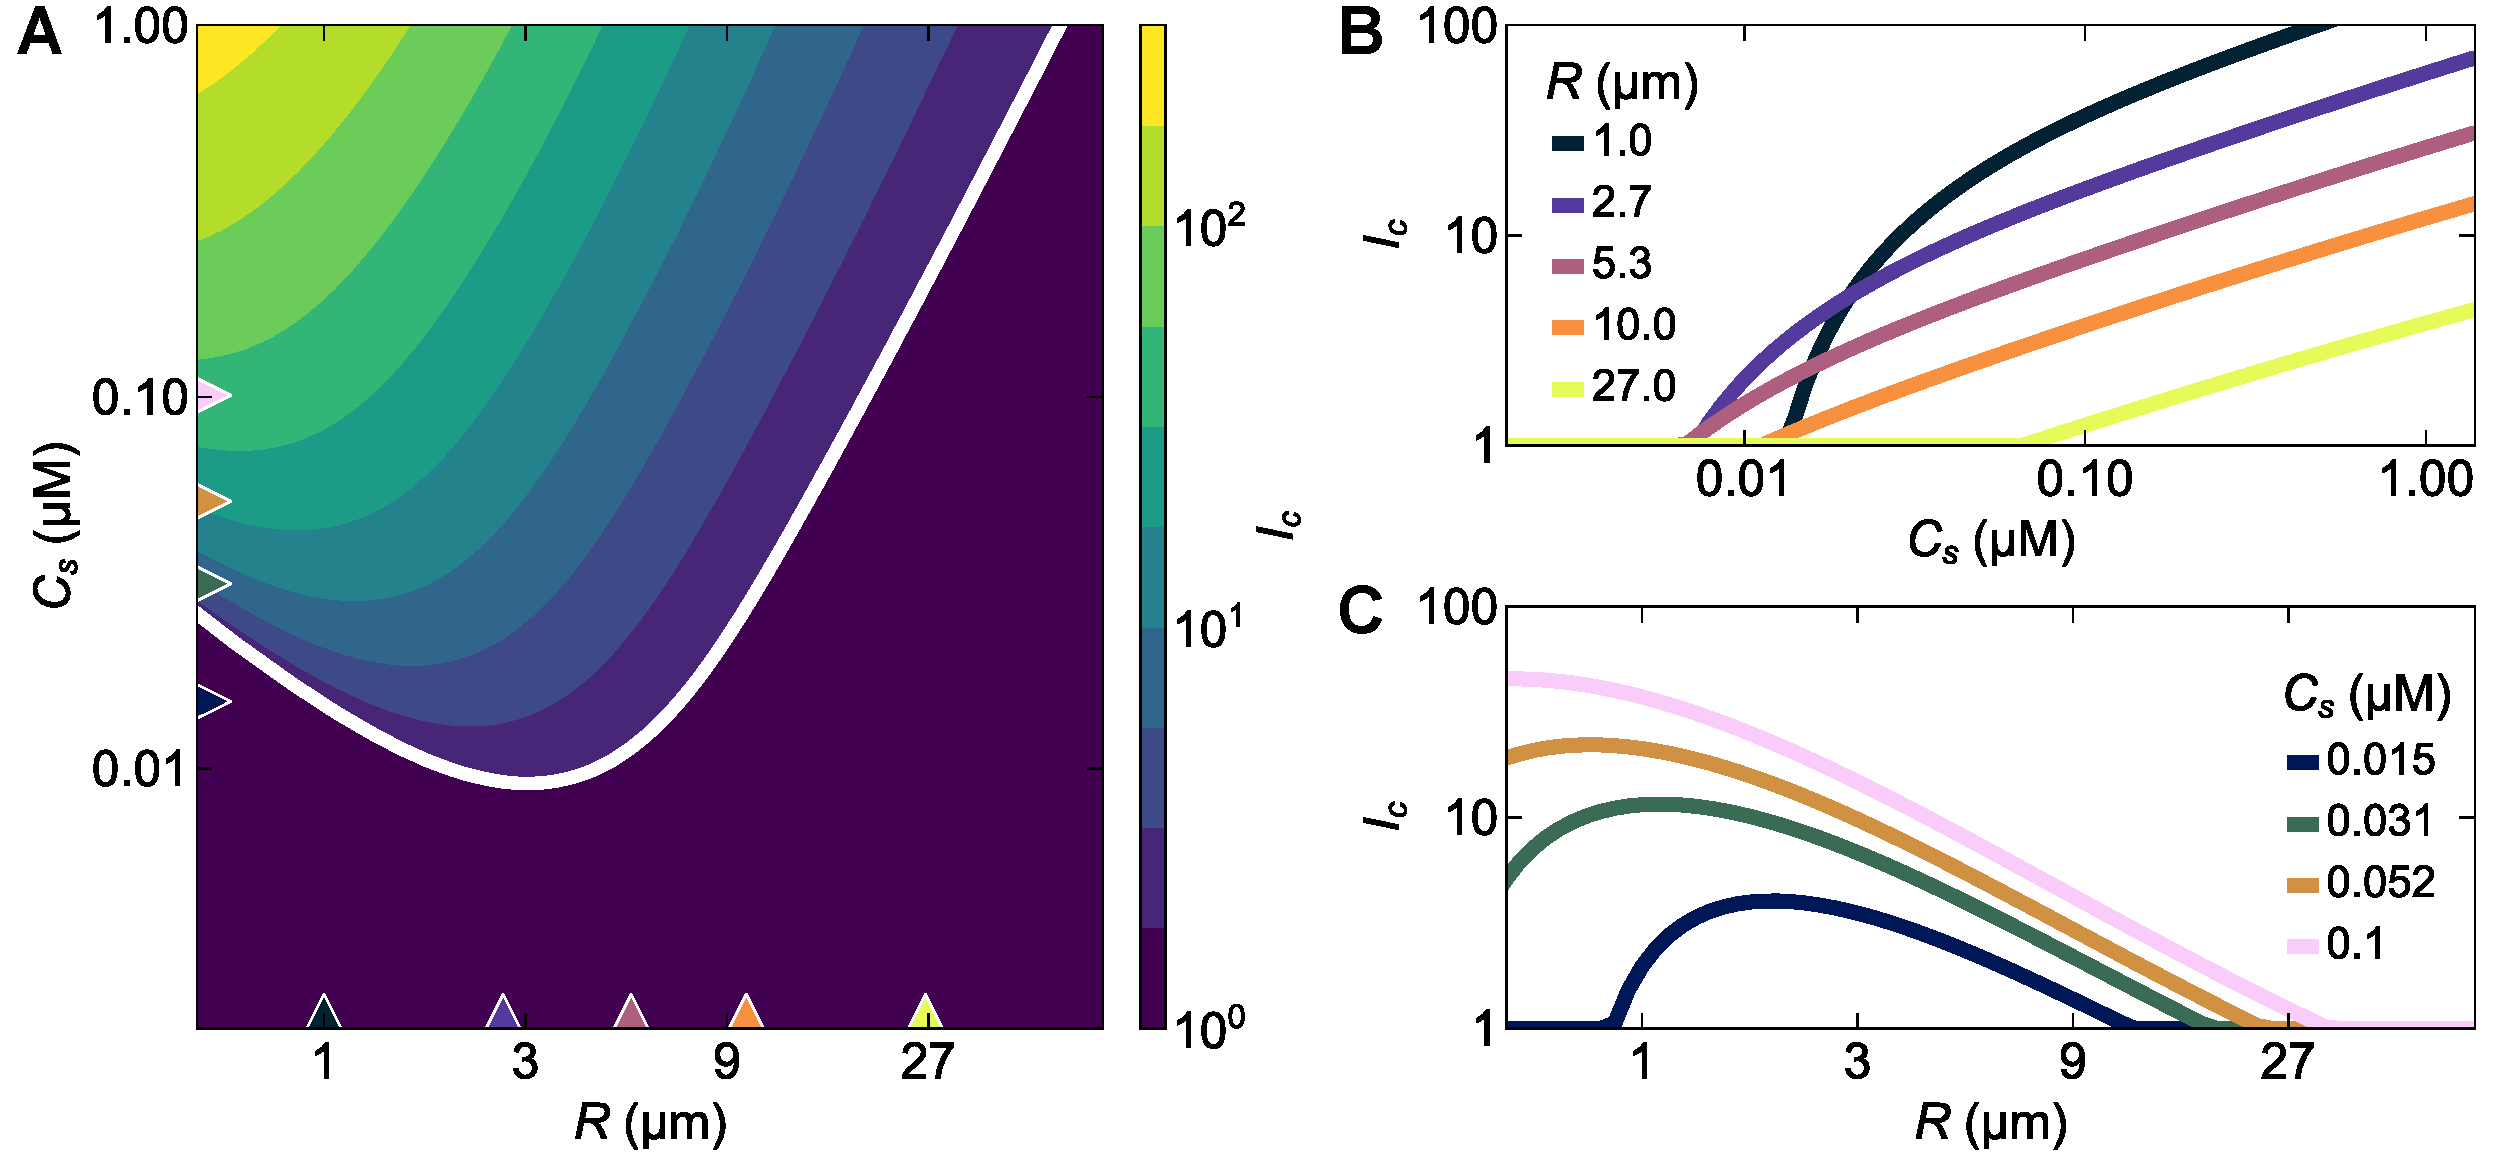
\includegraphics[width=17.8cm]{fig3_mod.pdf}
    \caption{
        \textbf{
        %The stakes are high for encounters with small phytoplankton -- the slope of the chemotactic index is steep for small but gentle for large phytoplankton.
        The stakes are high for encounters with small phytoplankton -- the chemotactic index is largest for small phytoplankton, but it drops sharply when gradient detection fails.
        %Asymmetrically steep performance landscape for chemotactic encounters - the stakes are higher for small phytoplankton.
        }
        (A) Performance ($I_c$) landscape for a bacterium using chemotaxis to drive encounters with spherical targets of different radii ($R$) and chemoattractant concentrations ($C_s$) calculated based on Eq. ??.
        % DB: Missing equation number.
        % DB: It could be worth writing the variable name on the axes for panel A, e.g., "Target radius R (µm)".
        The thick white line defines the boundary of detection, separating the region where gradients are detectable and chemotaxis is beneficial to encounters ($I_c > 1$) from the region where gradients are too shallow or too spatially confined to be detected ($I_c = 1$).
        %The sensing region is defined by the existence of a sensory radius $S>R$, as determined by the condition that the signal-to-noise ratio be larger than 1 (Eq.~\ref{}).
        %The thick white line ($S=R$) delimits the boundaries of detection.
        %For each $(R, C_s)$ within the sensing region, the $I_c$ of a perfect chemotaxer is evaluated using Eq.~\ref{}.
        %Small cells allow greater chemotactic performance due to the ballistic scaling of the encounter rates ($S^2/R^2$) compared to the diffusive scaling of large cells ($S/R$). 
        (B) Vertical transects from panel $A$ for fixed values of the target radius $R$ (corresponding to the upward-pointing triangles).
        In chemotaxis towards small targets, a slight variation in the chemoattractant concentration can make the difference between a highly successful search ($I_c\sim10$) or a failure ($I_c=1$), whereas for larger targets the dependency of $I_c$ on the chemoattractant concentration is more gradual.
        %The $I_c$ for chemotaxis towards small targets increases sharply as a function of the target concentration $C_s$, whereas the increase is more gradual for larger targets.
        (C) Horizontal transects from panel $A$ for fixed values of the chemoattractant concentration $C_s$ (corresponding to the right-pointing triangles).
        For weak sources, an increase in size $R$ produces initially large enhancements in chemotactic performance, with diminishing returns upon further enlargement.
        As the source gets stronger, the increase in performance for chemotaxis towards small targets becomes disproportionately larger; larger sources also become detectable although offering modest performance improvements over random searches.
        %As the concentration increases, the $I_c$ curves are more strongly skewed towards low-$R$ values.
        %Crossing the boundary of detection leads to large $I_c$ variations for spatially confined gradients, but only moderate variations for shallow gradients.
    }
    \label{fig:asymmetric-performance}
\end{figure*}


Chemotaxis towards small phytoplankton cells can be risky but highly rewarding.
%The performance landscape for chemotactic bacteria-phytoplankton encounters has a convex landscape and displays clear qualitative differences between the small-radii and the large-radii region (Fig.~\ref{fig:asymmetric-performance}A).
%A bacterium navigating straight towards the source of the stationary chemoattractant field $C(r)$ would experience a signal equal to the convective derivative of the field, $-U\dv*{C}{r}$, subject to an intrinsic noise~\cite{mora2010limits,brumley2019bacteria} $\sigma \approx 6\sqrt{3C(r)/(\pi a D_c T^3)}$. 
%for which we use the expression by Mora and Wingreen~\cite{mora2010limits} (augmented by the chemotactic precision factor $\Pi$ introduced by Brumley et al.~\cite{brumley2019bacteria}) $\sigma = \Pi \sqrt{3C(r)/(\pi a D_c T^3)}$.
%Defining $\mathrm{SNR} = -U\dv*{C}{r} / \sigma$, setting the detection threshold for Eq.~\ref{snr_general} to $q=1$ and using a cutoff function $f_\text{c}(x) = 1-\exp(-x^{3/2})$, we obtain a performance landscape for chemotactic bacteria-phytoplankton encounters which displays clear differences between the small-radii and the large-radii region (Fig.~\ref{fig:asymmetric-performance}A).
Application of our model to a ``typical'' marine bacterium (radius $a=\SI{0.5}{\micro\m}$, swimming speed $U=\SI{50}{\micro\m\per\s}$, sensory timescale $T=\SI{100}{\milli\s}$) chemotactic towards some sugar-like compound (diffusivity $D_c=\SI{500}{\micro\m^2\per\s}$) yields a quantitative description of the chemotactic performance landscapes which shows clear differences between the small-radii and the large-radii region (Fig.~\ref{fig:asymmetric-performance}A).
Here we assume the background concentration of the compound ($C_0$ in \autoref{chemoattractant_field}) to be fixed at \SI{1}{\nano M}, a value on the low-end for dissolved free amino acids in ocean waters~\cite{lee1975amino}. The effect of changing background concentration is discussed in the SI.
Contour lines of the $I_c$ profile have a higher density close to the detection boundary in the region of small phytoplankton radii, suggesting that modest variations in the excess concentration $C_s$ leaked by a small phytoplankter can have large impacts on the performance of bacterial chemotaxis.
Indeed, the $I_c$ has a much sharper dependency on $C_s$ when the phytoplankton radius $R$ is small, and especially so when crossing the detection boundary (Fig.~\ref{fig:asymmetric-performance}B): while a bacterium might not be able to sense ($I_c=1$) an attractant gradient from a \SI{1}{\micro\m} phytoplankter leaking with $C_s=\SI{10}{\nano M}$, a few \si{\nano M} increase can quickly enhance the $I_c$ to values of 10 and more; as $C_s$ is further increased we get deeper into sensing territory, and the dependency of $I_c$ on $C_s$ quickly smooths out.
For larger phytoplankton cells, there is no sharp increase: when the boundary of detection is crossed, the $I_c$ only grows gradually with $C_s$.
Simultaneously, for small values of the excess concentration $C_s$, an increase in phytoplankton radius $R$ leads first to a sharp increase in chemotactic index and then a gradual decrease towards $I_c=1$ when $R$ overcomes an optimal value (Fig.~\ref{fig:asymmetric-performance}C). As $C_s$ is increased, phytoplankton cells with smaller sizes keep offering disproportionately larger advantages to chemotactic performance compared to the larger cells whose detection requires larger and larger values of $C_s$.





\begin{figure*}
    \centering
    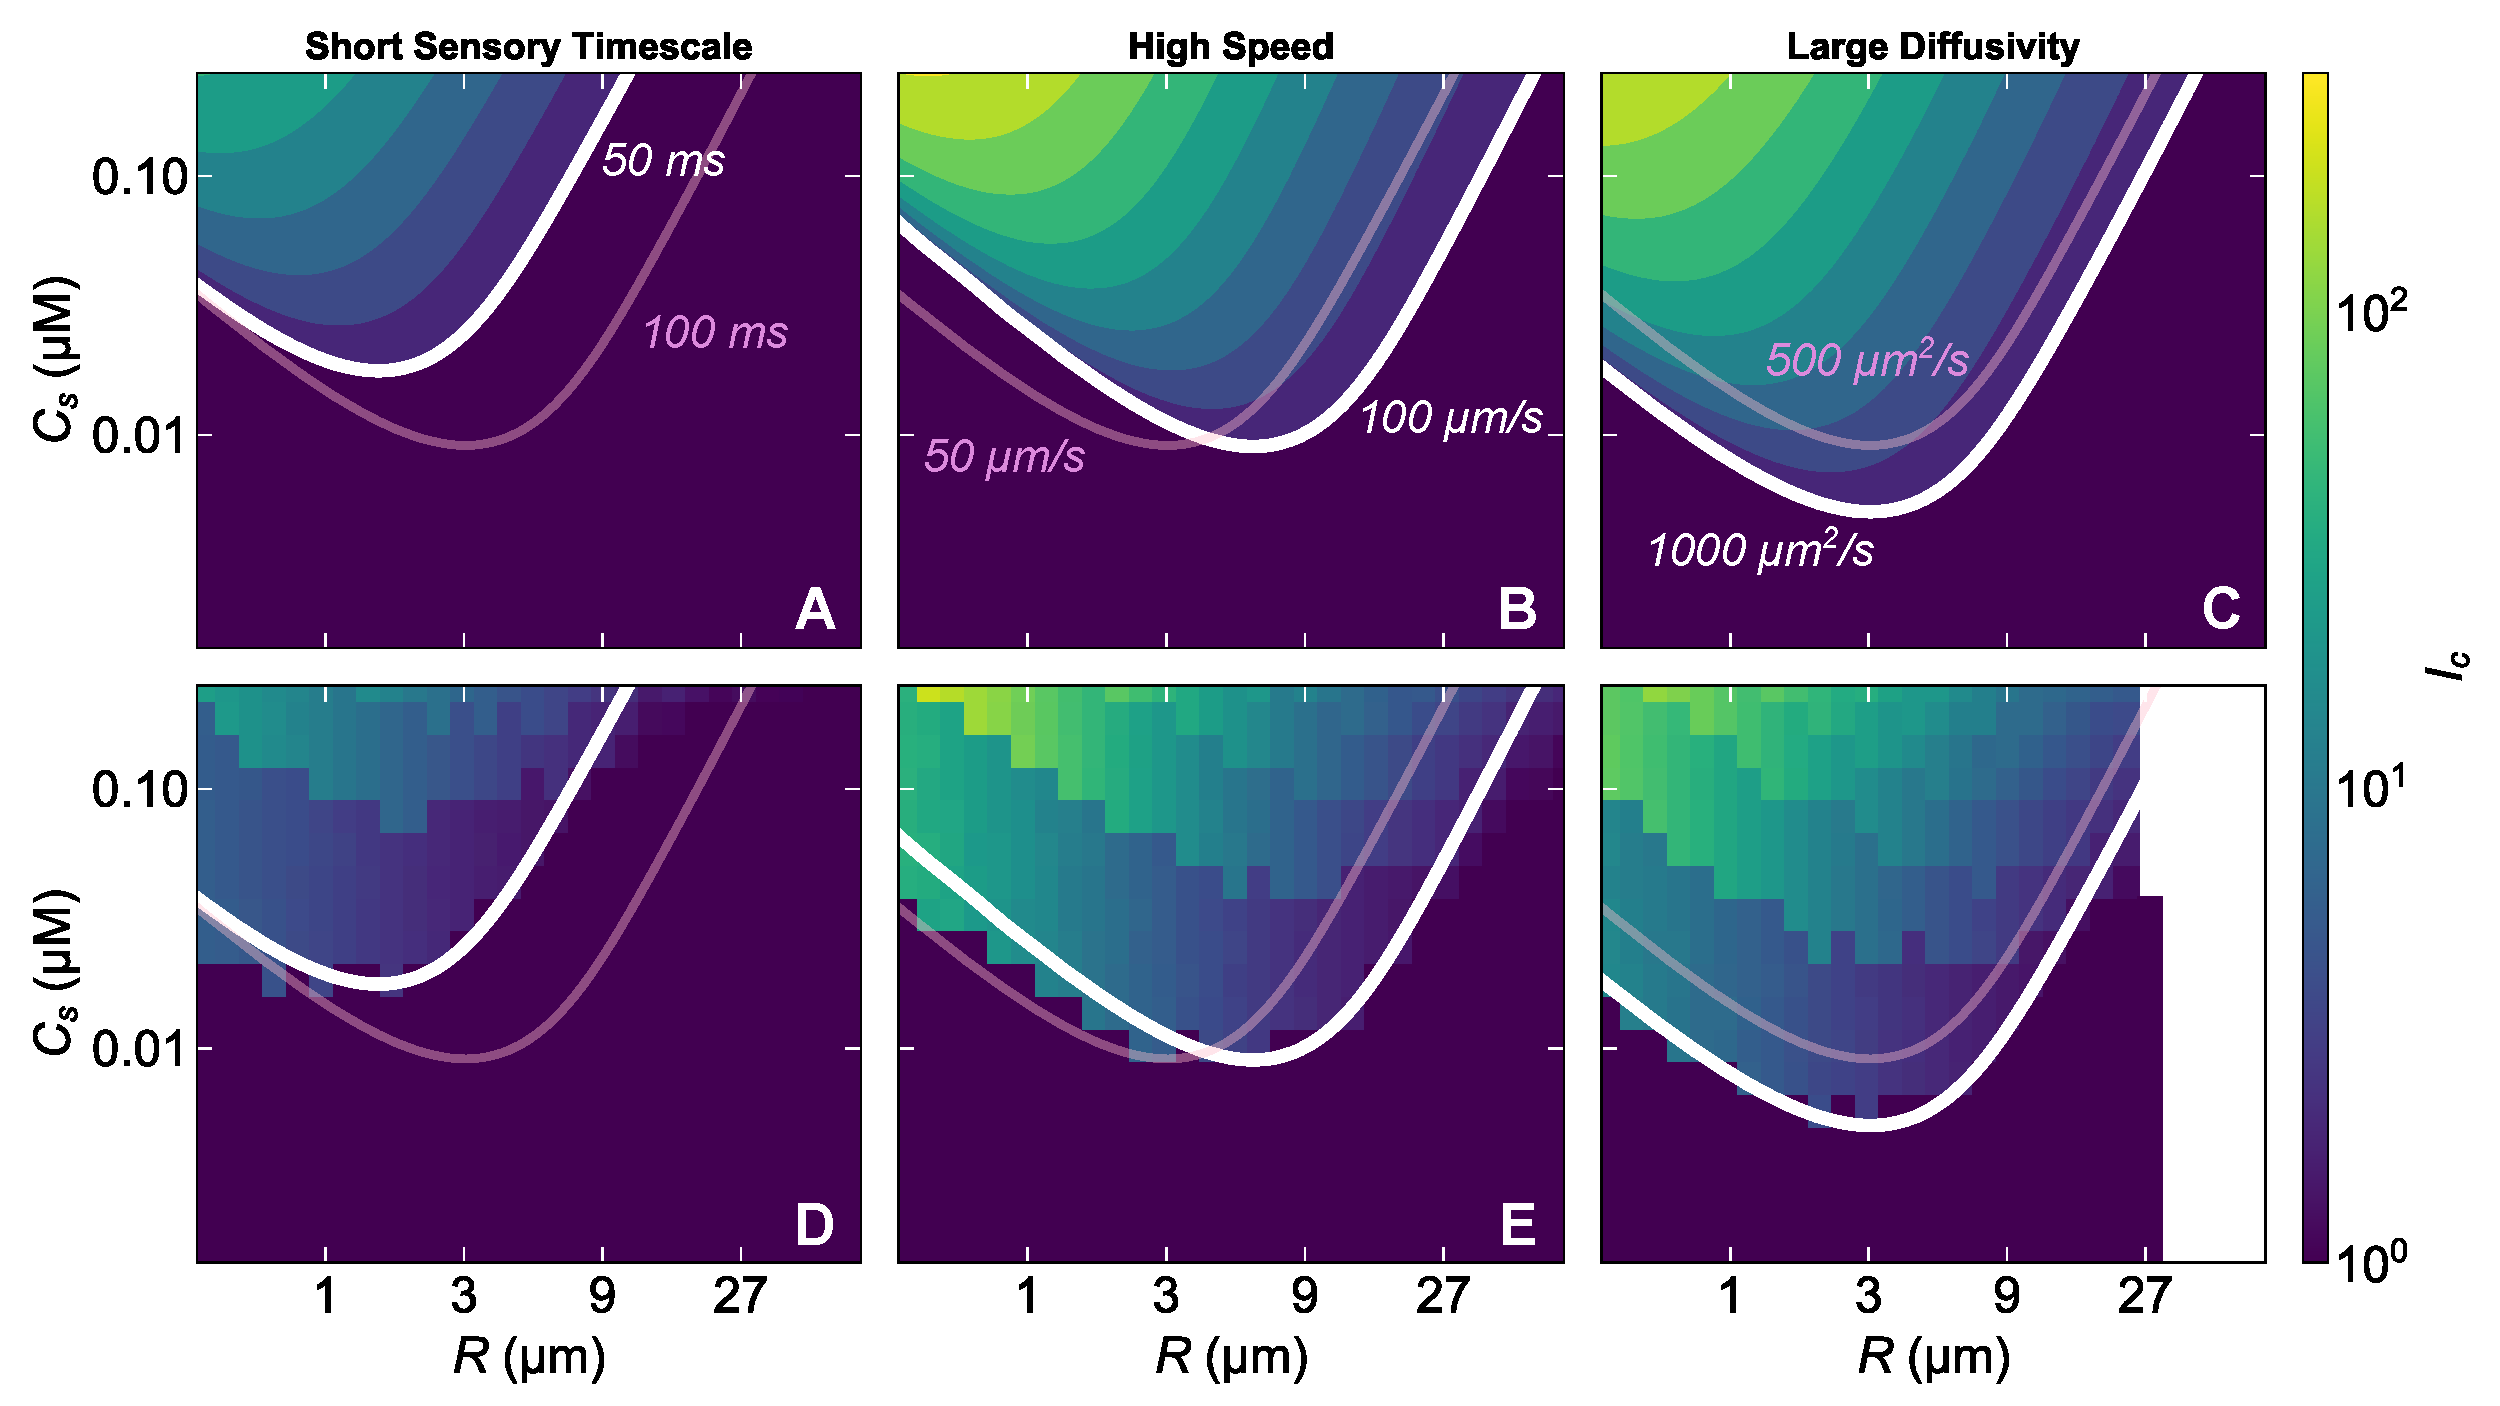
\includegraphics[width=17.8cm]{fig4_mod.pdf}
    \caption{
        \textbf{
        Bacterial chemotactic strategy controls the chemotactic index but does not alter the high-stakes nature of encounters with small phytoplankton.
        %Sensory timescale, swimming speed and chemoattractant diffusivity determine chemotactic performance, irrespective of the signal processing mechanisms.
        }
        Performance landscapes of different chemotactic strategies obtained from theoretical (A--C) and computational (D--F) models.
        In all the panels, the pink curve is the detection boundary for a reference strategy with parameter values $U=\SI{50}{\micro\m\per\s}$, $T=\SI{100}{\milli\s}$, $D_c=\SI{500}{\micro\m\per\s^2}$ (same as in Fig.~\ref{fig:asymmetric-performance}A).
        (A) Reduction in sensory timescale $T$ from \SI{100}{\milli\s} to \SI{50}{\milli\s}.
        (B) Increase in swimming speed from \SI{50}{\micro\m\per\s} to \SI{100}{\micro\m\per\s}.
        (C) Increase in chemoattractant diffusivity from \SI{500}{\micro\m^2\per\s} to \SI{1000}{\micro\m^2\per\s}.
        %(A) Both the sensing region and the chemotactic index respond to changes in the parameters.
        %The pink curve shows the boundary of detection for baseline values of the physical parameters ($T=\SI{100}{\milli\s}$, $U=\SI{50}{\micro\m\per\s}$, $D_c=\SI{500}{\micro\m^2\per\s}$) corresponding to the phase diagram of Fig.~\ref{fig:asymmetric-performance}.
        %Panels A-C show how the performance changes for a change in the sensory timescale (VALUE??) (A), swimmning speed (VALUE??) (B) and ... (C), relative to these baseline values. In the three columns shown here, we changed one parameter at a time compared to this reference, respectively:
        %$T=\SI{100}{\milli\s}$ to $T=\SI{50}{\milli\s}$;
        %$U=\SI{50}{\micro\m\per\s}$ to $U=\SI{100}{\micro\m\per\s}$;
        %$D_c=\SI{500}{\micro\m^2\per\s}$ to $D_c=\SI{1000}{\micro\m^2\per\s}$.
        (D--F) Theoretically predicted features of bacterial chemotactic performance are reproduced by an ideal sensor based on the Kolmogorov-Smirnov test.
        In panels D to F, the white line is the detection boundary from the theoretical prediction of panels A to C, respectively.
        Despite small quantitative differences in the estimated $I_c$ values, arising from the distinct signal processing mechanism and the finite spatial resolution of numerical simulations,
        the features of the performance landscape are clearly conserved.
        % DB: My first impression from the bottom panels D-F is that there is some noise or computational limitations for the computational model. It seems a little strange that the value of I_c seems to have rather strong discontinuities as C_s is increased. However, I then realised that you have probably thresholded the data to have discrete colours (as in the top row). I understand this is done to match exactly the approach for the top row, but I think it makes the computational model look noisy and irregular. Have you considered using a smooth colour map (for all 6 plots), but placing very find contour lines for the values of interest? This will give you a smooth colourmap but with curves to guide the eye. We did this in the NanoSIMS paper (https://stockerlab.ethz.ch/wp-content/uploads/2023/02/161.Chemotaxis-increases-metabolic-exchanges.pdf) in Figs. 3-4 and it worked quite well.
        %
        % DB: Also, for me half of panel F is missing (even when the PDF is downloaded). Are there computational limitations there?
    }
    \label{fig:strategies}
\end{figure*}



Variations in chemotactic search strategies, defined by parameters such as swimming speed $U$, sensory timescale $T$ or diffusivity of the sought-for compound $D_c$, determine the benefits of chemotaxis for a given phytoplankton radius and excess concentration, but do not affect the fundamental structure of the performance landscape (Fig.~\ref{fig:strategies}).
A reduction in sensory timescale from $100$ to \SI{50}{\milli\s} significantly decreases bacterial ability to detect gradients from large phytoplankton cells and reduces the overall performance of chemotaxis (Fig.~\ref{fig:strategies}A): a larger $T$ reduces sensing noise ($\propto T^{-3/2}$) but increases dynamic noise by reducing the frequency of measurements.
An increase in swimming speed from $50$ to \SI{100}{\micro\m\per\s} improves the performance of chemotaxis within the region of detectability, but the region itself is shifted towards larger radii values, highlighting a tradeoff between degraded spatial resolution (lower frequency of measurements) and improved sensing accuracy by reducing bias in the signal~\cite{hein2016physical}(Fig.~\ref{fig:strategies}B).
An increase in the diffusivity of the chemoattractant compound from $500$ to \SI{1000}{\micro\m^2\per\s} 
% DB: Very minor comment: some units are "/s" and others are "s^{-1}". It's probably worth unifying throughout.
(values similar to the diffusion coefficients of sugars and DMSP respectively~\cite{})
% DB: missing reference. We have references buried in the SI for our 2019 paper that could be useful for calculating the diffusion coefficients
enhances the signal-to-noise ratio without affecting spatial resolution (sensing noise $\propto D_c^{-1/2}$), and it thus shifts the region of detectability towards lower $C_s$ values (Fig.~\ref{fig:strategies}C).
Unaffected by the variation in these quantities, the high-stakes nature of chemotactic searches towards small phytoplankton cells is therefore only a direct result of the sharp cutoff on spatial resolution arising from dynamic noise combined with the quadratic scaling of the $I_c$ associated to ballistic encounters.

The generality of our theoretical analysis is supported by a numerical model of an ideal sensor which has no direct relationship 
% DB: Rather than saying "no direct relationship" (which comes across as tangential or unlrelated), I would suggest rephrasing to mention "minimal model", or something that distils the essential features of chemotaxis without needing to specify actual pathways.
to bacterial chemosensory mechanisms (Fig.~\ref{fig:strategies}D--F).
This ideal sensor is defined as a sphere moving at constant speed $U$ towards a phytoplankton cell leaking a chemoattractant field $C(r)$.
As it moves, the sensor registers all the adsorption events of chemoattractant molecules, occurring as Poisson events with instantaneous rate $4\pi D_c a C(r)$.
After an interval of length $T$, the registered events are processed and a new acquisition starts.
For the signal processing, the sensor performs a one-sided Kolmogorov-Smirnov test~\cite{massey1951kolmogorovsmirnov} comparing the distribution of the waiting times recorded in the first and the second half of the acquisition window.
If the cumulative distribution function in the second half is found to be larger than that in the first half, then the sensor has detected a gradient. Averaging the successful gradient detections over an ensemble ($N=1000$) 
% DB: Is this number based on particular convergence tests? Have you also considered averaging over different angles, or only taking the 'direct approach'?
of such ideal sensors provides an estimate of the sensory distance $S$, defined as the largest distance where at least a fraction $f$ of the sensors has detected a gradient. The estimates of $S$ can then be used to evaluate the chemotactic index $I_c$.
Remarkably, we find that choosing a high consensus threshold $f=0.99$ provides close agreement with our theoretical calculations, both in terms of the shape of the detectability region and of the estimated $I_c$ values.
This fact highlights how the detection limits evaluated for bacterial chemosensing and the asymmetric nature of the chemotactic performance are not specific to bacteria, but can be used to describe a wide class of systems estimating gradients through temporal comparisons, independently of the particular signal processing mechanism and navigation parameters.
% DB: very nice!



%Section 'Search timescales in realistic conditions'.


\begin{figure*}
    \centering
    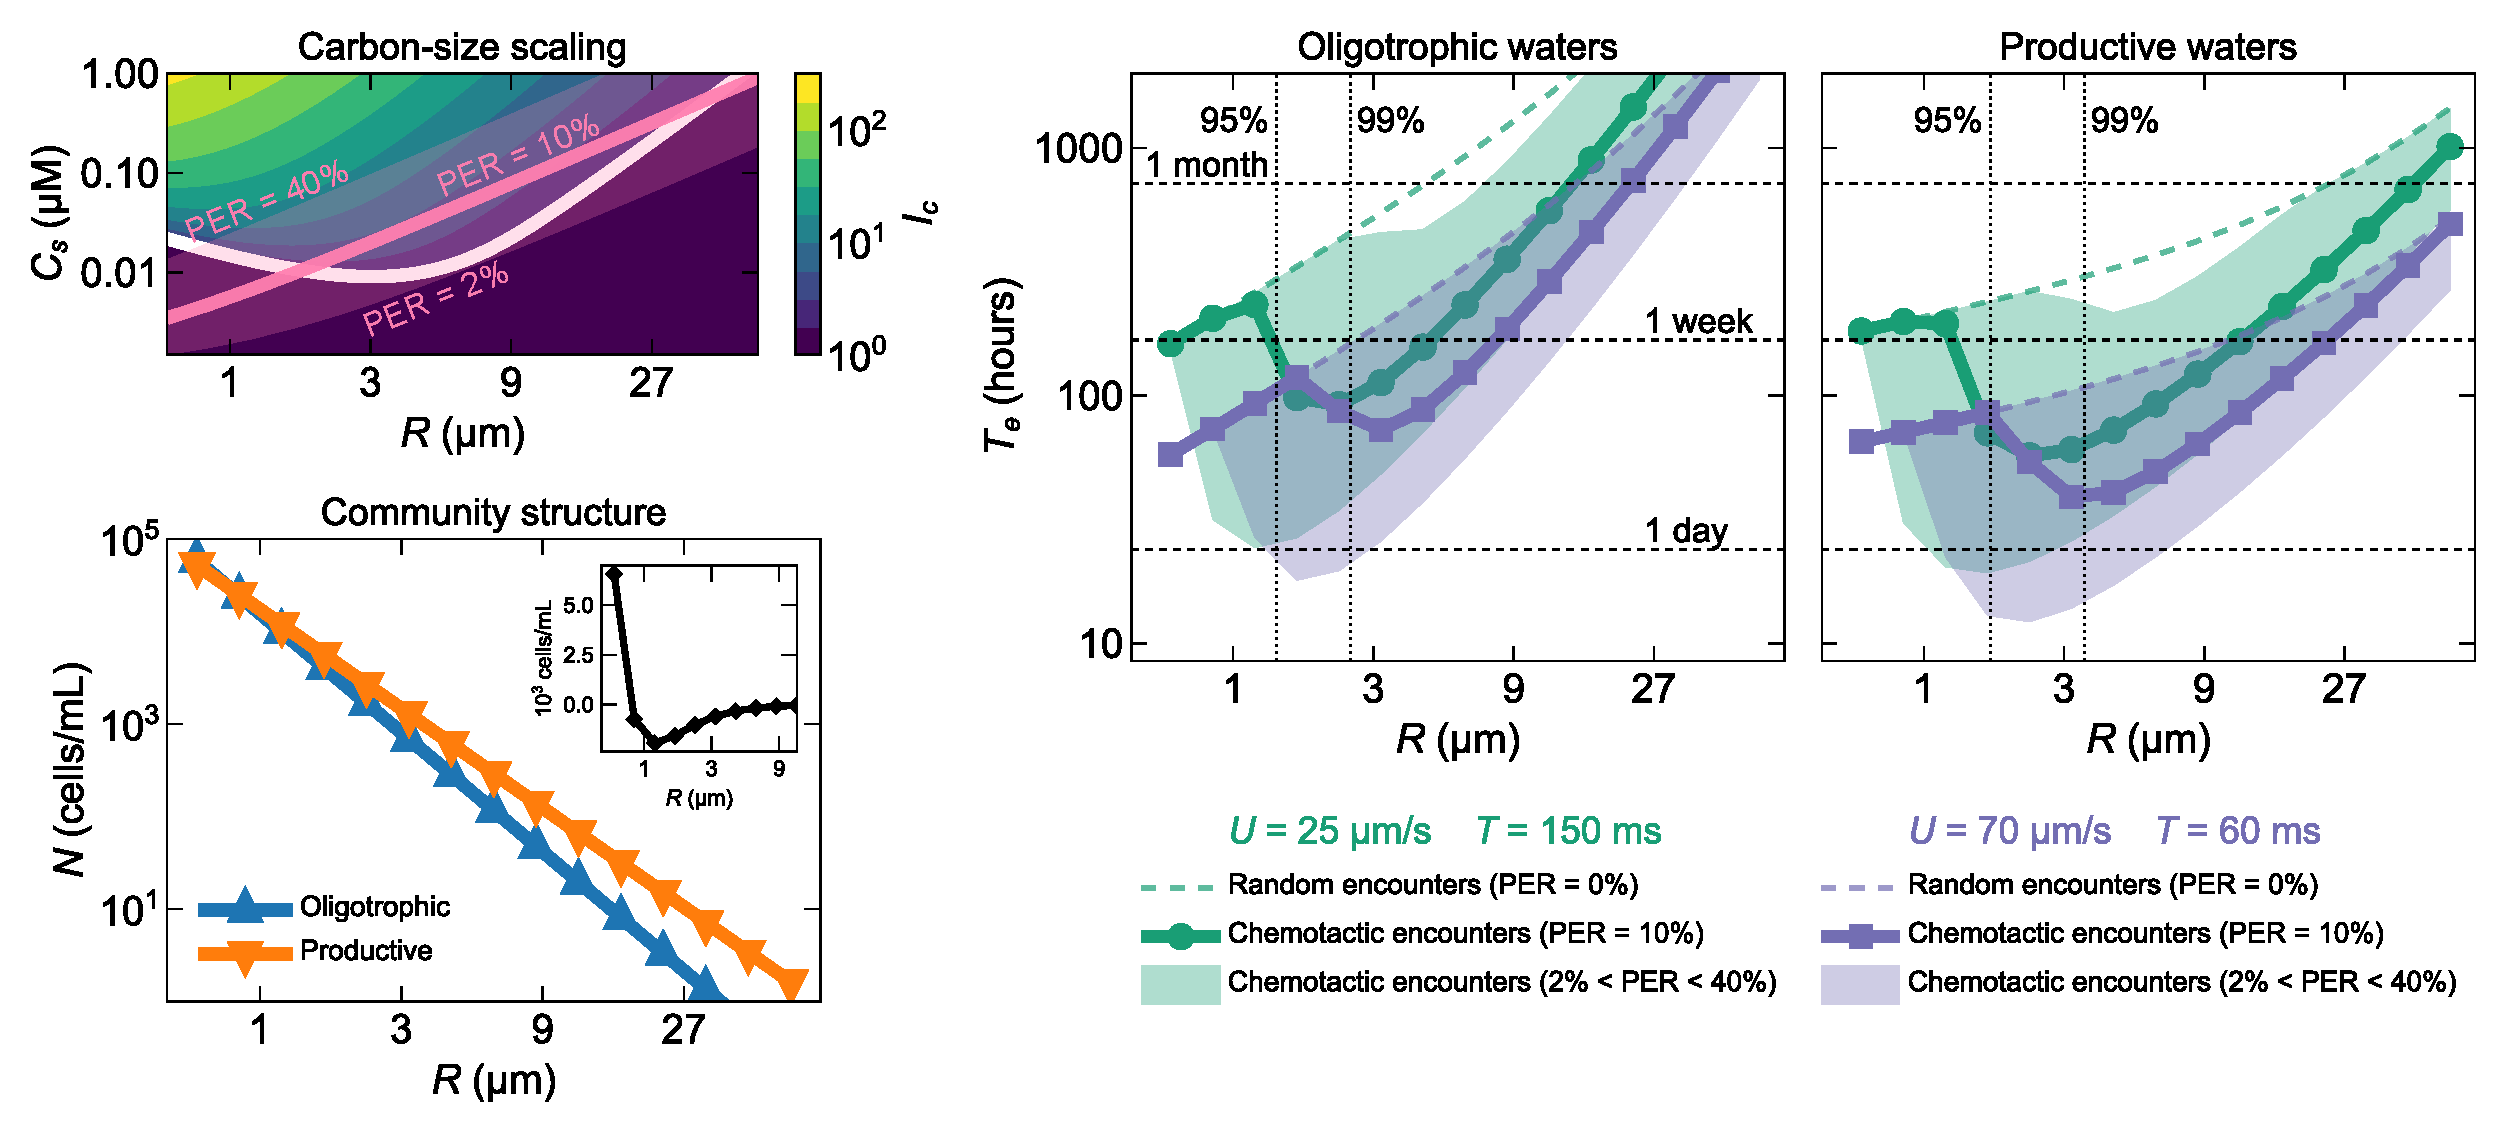
\includegraphics[width=17.8cm]{fig5_mod.pdf}
    \caption{
        \textbf{
        The high-stakes nature of phytoplankton-bacteria interactions may promote a diversity of chemotactic strategies.
        }
        %Ten-fold reduction in search times for the smallest phytoplankton cells may require bacteria to move slower and increase their sensory timescale.}
        %Chemotaxis can decrease search times by an order of magnitude, but detection of smaller targets 
        %We compute chemotactic performance towards targets with size distribution and leakage rates that mimic typical marine phytoplankton communities.
        %(A) Classical carbon-size relationships define the region of $R-C_s$ space accessible to bacteria-phytoplankton interactions (pink band).
        %The $I_c$ landscape was evaluated for a bacterium with $U=\SI{50}{\micro\m\per\s}$, $T=\SI{100}{\milli\s}$ and a chemoattractant diffusivity $D_c=\SI{500}{\micro\m\per\s^2}$.
        (A) Characteristic values of size and released chemoattractant for phytoplankton cells are constrained by carbon-size scaling laws (pink areas). When overlaid on the performance landscape of a bacterium (same as in Fig.~\ref{fig:asymmetric-performance}A), the physiological range of exudation rates lies across the boundary of detection.
        The thick pink line corresponds to phytoplankton cells with a percent extracellular release (PER) of 10\%, the shaded pink band represents variations in the percent extracellular release between 2\% (lower limit) and 50\% (upper limit).
        % DB: I added "PER" in brackets since this is used in the figure panel.
        %
        % DB: Can you add the labels A, B, C, D to the figure image?
        %
        %The WHICH COLOR? band highlights the region with percent extracellular release (PER) between 2\% and 50\%, with the thick pink line representing a typical value of 10\%.
        %For all phytoplankton cell radii $R$, chemotaxis has the possibility to enhance encounters, but the region of extremely high $I_c$ ($>100$) will not be accessible in typical conditions.
        (B) Marine phytoplankton communities are dominated by small cells. The size structure follows a power-law distribution, where the abundance $N$ decreases with increasing size $R$ as $N(R) \propto R^{-3\alpha}$.
        The allometric exponent is larger in oligotrophic waters ($\alpha\simeq 0.9$) than in more productive waters ($\alpha\simeq 0.75$). Both  communities are normalized to a total cell abundance of \SI{1e5}{cells/\milli\liter}.
        %The smallest size classes are therefore more abundant in oligotrophic waters (difference between oligotrophic and productive abundances shown in inset).
        Inset: difference between cell abundance in oligotrophic and productive waters.
        % DB: I suggest putting a dashed line for the zero value in the inset figure.
        (C-D) Comparison of search times between random motility and chemotaxis.
        Carbon-size scaling, phytoplankton community structure and chemotactic index jointly define the average search time ($T_e$) (Eq.~\ref{eq:search_time}) an individual bacterium requires to encounter a phytoplankton cell using chemotaxis.
        % DB: Maybe explicitly say that this is the average time.
        The thin broken lines represent the search times in the absence of chemotaxis ($I_c=1$).
        The thick lines with markers indicate search times for phytoplankton cells with percent extracellular release of 10\% (corresponding to the thick pink line in panel A), and the shaded bands represent variations in percent extracellular release between 2\% and 50\% (matching the pink shaded band in panel A).
        The two curves correspond to distinct chemotactic strategies: in green with circle markers, a strategy with low speed and long sensory timescale; in violet with square markers, a strategy with high swimming speed and short sensory timescale.
        The vertical dotted lines mark the radii corresponding to the 95\textsuperscript{th} and 99\textsuperscript{th} percentiles of the phytoplankton community abundance.
        % DB: Is it possible to move the "1 month" label to the right hand side of panel C, in keeping with the other labels?
        %
        %Colored bands highlight the range of possible values according to the accessible region shown in panel A. The thick lines with markers correspond to $\text{PER}=10\%$.
        %Larger swimming speeds improve random search times at the cost of giving up sensing on the smallest cells.
        %The vertical dotted lines denote the 95th percentile of the phytoplanktonpopulations, highlighting that, in both environments, the vast majority of phytoplankton cells lies below the $\SI{2}{\micro\m}$ radius.
    }
    \label{fig:ecology}
\end{figure*}


%While our theoretical investigation has provided general insight about the behavior of encounters assisted by chemosensory mechanisms over a broad range of radii $R$ and excess concentration values $C_s$, phytoplankton cells will only be found in a limited region of values.
%Using empirical carbon-size scaling laws~\cite{mullin1966relationship,menden-deuer2000carbon}, each phytoplankton cell size $R$ can be associated to a given carbon content. At any time, a fixed fraction of the total carbon content of the cell, termed the percent extracellular release (PER), is assumed to be exuded with a constant rate, which then defines the value of the excess concentration at surface $C_s$.

The physiological range of exudation rates for healthy phytoplankton cells lies across the boundary of chemotactic detection (Fig.~\ref{fig:ecology}A), suggesting that chemotaxis might play a relevant role for encounters across the entire size spectrum. The physiology of marine phytoplankton enforces a specific coupling between size $R$ and excess concentration $C_s$.
Empirical carbon-size scaling laws predict that the carbon content of a cell scales with cell size as $\sim R^{2.28}$~\cite{mullin1966relationship}; the percent extracellular release (PER) then determines how much of this total content is leaked to the environment (SI).
Average values of the PER are expected to be around 10\%, but variations between values of $\mathrm{PER}\approx 2\%$ and $40\%$ are typical and also strongly dependent on physiological and environmental conditions~\cite{maranon2004significance}.


%In addition to the increase in encounters provided by chemotaxis as measured by the chemotactic index $I_c$, we want to estimate the actual rate at which such encounters occur in the ocean, or equivalently, the average time a bacterium needs to search before encountering a phytoplankton cell.
%The steep size-structure of phytoplankton communities regulates encounters across the size spectrum.
The steep size-structure of marine phytoplankton communities favors encounters with small phytoplankton cells.
The average search time required by an individual bacterium to encounter a phytoplankton cell can be obtained as
\begin{equation}\label{eq:search_time}
    T_e = \dfrac{1}{I_c \Gamma N}
\end{equation}
where $\Gamma$ is the random encounter kernel between the bacterium and the phytoplankton and $N$ is the phytoplankton concentration.
% DB: It could be worth mentioning the units of the encounter kernel. Also possibly cite a reference for this (e.g., Thomas Kiorboe's book).
Marine phytoplankton communities have characteristic size structures which usually follow a power-law size-abundance relationship of the form $N(R) \propto R^{-3\alpha}$, where the allometric exponent $\alpha$ takes typical values $\alpha\approx0.9$ in oligotrophic waters and $\alpha\approx0.75$ in productive waters~\cite{cermeno2008species}.
Phytoplankton cells with smaller radii are therefore vastly more abundant than cells with larger radii, and particularly so in oligotrophic environments where large phytoplankters are extremely rare (Fig.~\ref{fig:ecology}B).
This peculiar size-structure allows bacterial search times for small phytoplankton cells to be much shorter than those for larger cells.
% DB: Why is this peculiar?
%
The overabundance of small cells, combined with the asymmetric performance landscape of bacterial chemotaxis, further raises the stakes for chemotactic searches in the low end of the size spectrum.

%The steep size-structure of phytoplankton communities clearly favors encounters with the smaller phytoplankton even in the absence of chemotaxis (Fig.~\ref{fig:ecology}C--D, thin lines).
Chemotaxis significantly reduces search times in the sub-\SI{5}{\micro\m} range, but different chemotactic strategies can display dramatic performance differences in the low end of the spectrum (Fig.~\ref{fig:ecology}C--D).
% DB: The panels in Fig. 5 are not labelled A, B, C, D.
In the absence of chemotaxis, small phytoplankton cells require much shorter search times than large phytoplankton (Fig.~\ref{fig:ecology}C--D, thin broken lines).
In oligotrophic waters, a bacterium swimming randomly with speed \SI{40}{\micro\m\per\s} can encounter a phytoplankton of radius $0.5\sim\SI{0.7}{\micro\m}$ roughly every $100$ hours, while encountering a phytoplankton in the range $24\sim\SI{33}{\micro\m}$ will take on average more than a month. 
% DB: For these size ranges above, I think it would be better to use "-" than "\sim".
%
In productive waters the search times for small cells are only slightly higher, whereas those for larger cells fall down below a month. Bacteria with a higher swimming speed of \SI{80}{\micro\m\per\s} reduce their random search times due to improved exploration efficiency, although that comes with a tradeoff in terms of chemotactic performance, as also shown in Fig.~\ref{fig:strategies}B.
The decreases in search times resulting from the use of chemotaxis, over the whole range of phytoplankton PER values, are shown as shaded bands in Fig.~\ref{fig:ecology}C and D, with the thick marker-decorated line representing the typical value $\mathrm{PER}=10\%$.
Bacteria with lower speed but longer sensory timescales $T$ can decrease their search times for the smallest phytoplankton almost by a factor 10, whereas the faster swimming bacteria with a shorter sensory timescale cannot benefit at all from chemotaxis at this extreme of the spectrum.
%The importance of this apparently tiny difference (as seen by the difference in the green and violet bands of Fig.~\ref{fig:ecology}C and D), is better understood by realizing that the smallest cells constitute the vast majority of the population.
While the major difference in the $I_c$ between the two strategies is limited to the micron-size range, we stress that this region of the size-spectrum encloses the vast majority of the population.
The 95th percentile of the populations (marked by the dotted vertical lines in the figures) is below the \SI{2}{\micro\m} radius, and, in both environments, more than half of the population is contained within the first size class.
Therefore, losing the ability to increase encounters with the smallest cells in the spectrum can dramatically impact the dynamics and the fate of populations.
We must also note that the boost in chemotactic performance towards small cells occurs only at high PER, while no gain can be obtained with intermediate PER values; for the larger ($>\SI{2}{\micro\m}$) radii, the reduction in search times is more robust and occurs also at lower PER values.


%% diversity statement
%These rather general features of chemotaxis-assisted encounters may support and even promote the coexistence between generalist bacteria, with phenotypes better suited to increase encounters over the entire size spectrum, and specialist bacteria which optimize their performance in the low-end of the spectrum, where the competition is strongest.


% Discussion: paragraph on generality (this should also work for particles, maybe even the immune system); paragraph on how the 'high-stakes' could drive diversity of chemotactic strategies beyond gradient ascend - this is due to the tension between gain due to ballistic encounter and limitation by gradient confinement.


%% Speculatory paragraph on evolutionary games - mention the growth return part of the game
Assuming the minimization of search times to be the end-goal of a cell, it is suggestive to think of the chemotactic encounter problem as an evolutionary game with a strongly asymmetric fitness function.
In this context, the $I_c$ can be interpreted as a measure of the maximum possible fitness attainable by a bacterium: it is possible to obtain huge fitness benefits in the search for small phytoplankton cells, but relatively small ones when searching for large cells. 
%The question then becomes: how close to the upper limit can bacteria really get? We can imagine that different bacteria, either as a result of genotypic or phenotypic diversities, will behave differently once inside the sensory horizon: specific behavioral responses can thus be interpreted as different ``implementations'' of chemotactic behavior; none of them can outperform the theoretical $I_c$ evaluated for the perfect chemotaxer but they will compete for survival. Any implementation will tend to perform better (i.e. closer to the theoretical optimum) in certain regions of parameter space, and worse in others.
%Now, is there a diversity of chemotaxis ``implementations'' in bacteria? It is known that phenotypical diversity exists~\cite{} but, regarding the existence of different \textit{behaviors}, the pragmatic answer seems to be negative, since we typically associate chemotaxis to a single well-defined behavioral response: a decrease in tumble rates when moving along positive gradients. How well does this implementation perform across the size spectrum?
%We also know, however, that other, sometimes minor, effects exist, such as... [examples chemotaxis+chemokinesis, is there some other known variation?]
We must keep in mind, however, that the encounter is only the initiating step of a possibly multi-stage interaction process and that fitness is determined by the ability to grow and reproduce. %, and that in nature, the goal is probably not just to encounter ``something'', but to encounter the most valuable resource. In some cases, we can expect that bacteria may not even care about a physical encounter with the source, as long as they can increase their residence time within the phycosphere.
To obtain a more complete eco-evolutionary picture, one would need to simultaneously consider the search time and the growth return associated to phytoplankton cells of different sizes. %, as postulated in the foraging mandala proposed by Fernandez \textit{et al}~\cite{}. Deeper analysis in this direction would require further assumptions on the exact nature of the bacterium-phytoplankton interaction (e.g. a mutualism only limited by the carrying capacity of the phytoplankton, an opportunistic interaction where the bacterium consumes the exuded compounds... ?) which are system-specific and go well beyond the scope of this work.
In fact, chemotaxis is expected to not only reduce search times, but to also (and most prominently) improve the growth returns, allowing bacteria to remain nearby local maxima of chemoattractants even without a direct encounter~\cite{fernandez2019foraging}.
Indeed, Raina \textit{et al.}~\cite{raina2023chemotaxis} have shown that \textit{Marinobacter adhaerens} can use chemotaxis to increase nutrient uptake (and therefore growth returns) from \textit{Synechococcus} cells, but they don't provide any information on whether chemotaxis also reduces the search times.
% DB: In the paper above, we showed that chemotaxis increases the (i) frequency of interactions with target cells (hotspots per day); and (ii) the residence time spent in the vicinity of a target. The former point does therefore imply that the search time is reduced using chemotaxis. In fact, chemotaxis gave a ~3 fold increase in overall encounter rate, which is commensurate with your estimate for the search time reduction in Fig. 5.
%
%Generally, it is expected that ``resource quality'' will increase with increasing cell size (e.g. proportionally to the total carbon content of a cell), thus at least partially offsetting the much shorter search times associated to small phytoplankton and further complicating the landscape.
%How the interplay between the size-dependence of chemotaxis-assisted search times and resource quality regulates the interaction landscape of the ocean is therefore an open point which warrants further study.
Further considerations on the growth returns should also include estimates of the energy expenditure associated with motility and chemotaxis~\cite{malaguti2021theory,keegstra2022ecological}, and the fact that foraging efficiency is typically positively correlated with predation risk~\cite{nielsen2021foraging}.

%% Limitations - dump everything here
Our work points to several potential extensions to better understand the role of chemotaxis in regulating encounters. The requirement to include multiple phenomena in our model (bacterial motility, dynamic and inherent noise in chemosensing, phytoplankton exudation, carbon-size scalings, community structures) clearly leads to simplifications which complicate the task of making explicit predictions, but our approach provides at least a framework in which the effects of chemotaxis on microscale interactions can be better understood. 
Explicit numerical simulations of chemotactic bacteria towards leaky phytoplankton cells could also help establish relationships between search times and uptake rates, and how these two quantities are simultaneously modulated by motile and chemotactic properties. Different chemoattractants (which we only considered through their molecular diffusivity) are also known to elicit wildly different chemotactic responses, especially when multiple chemical species are simultaneously present~\cite{clerc2023strong}, an effect which we are not able to include in our calculations.
Moreover, there is a clear need to design experiments to assess, at least in simple scenarios with single chemical species, how close to these theoretical limits bacteria can operate and if it is reasonable to tie the mathematical concept of the sensory horizon to the empirical notion of phycosphere~\cite{seymour2017zooming,bell1972chemotactic,platt2023probing}.
% DB: I think it is certainly already "reasonable" to do this, so would tune the language a bit. Maybe to examine the effect that truncating the response has, i.e. the thresholding process, as opposed to a continuous responses as a function of distance.



% DB: There are a few other points that could be good to include in the discussion section
%
% - Since the response is quite sensitive to changes in the leakage rate (e.g. through PER or size), it would be good to emphasise that community dynamics can change very abruptly through different seasonal cycles or bloom conditions. 
%
% - The functional form you have chosen for the nutrient profile (~1/r) is one specific choice, which neglects background consumption by bacteria. Do you have a rough sense for what would happen if you allowed for uptake, which would shape the profile to be like C(r)~exp(-k*r)/r. We used this form in the 2023 Nat. Microbiol. paper, since taking a superposition of 1/r sources doesn't converge. This would sharpen the gradients even further and possibly accentuate the findings of high stakes dynamics for small cells.
% JS: spatial profile of C(r) in general
%
% - The chemotactic sensitivity can change dramatically over time, as the bacterium's metabolism shifts. In addition to the phytoplankton changes (e.g., through PER and oligotrophic size distribution), it might be worth discussing the role of bacterial sensitivity changes. We discussed this point in the following paper, e.g. see Fig. 2: https://www.frontiersin.org/articles/10.3389/fmars.2020.00527/full. But perhaps this is beyond the scope of this paper.
%
% - The calculation that small phyoplankton are found more readily when bacteria swim slower, but have a longer value of T, relies on the assumption that the gradients are steady. I wonder if it is worth discussing/hypothesising what would happen if ephemeral patches are included.


%% Conclusions paragraph
%Using idealized models of phytoplankton leakage and bacterial chemotaxis, we have identified fundamental limits to the ability of bacteria to detect gradients and used them to establish upper bounds to the enhancement in bacteria-phytoplankton encounters driven by chemotaxis.
Using idealized models of phytoplankton leakage and bacterial chemotaxis, we calculated upper bounds on the enhancement in bacteria-phytoplankton encounters driven by chemotaxis over random motility, and studied how sensitive the enhancement is to the size of phytoplankton. We found that bacterial chemotaxis offers low-risk/low-gain performance for searches of large phytoplankton but high-risk/high-gain performance for small phytoplankton. These tradeoffs arise from chemotactic encounters being limited by fundamentally different mechanisms at the two ends of phytoplankton size spectrum. For large cells, the limitation stems from gradients' steepness and the diffusive nature of bacterial motility and leads to a moderate reduction in chemotactic search times. By contrast, for small phytoplankton, the limit is set by the gradients' spatial confinement and ballistic motility of bacteria, which, in principle, allows for nearly ten-fold reductions in search times provided that bacteria can detect the gradients. We found that searching for small phytoplankton is more efficient when bacteria swim slower but integrate the gradients over longer sensory timescales. Overall, our results suggest that the high-stakes nature of encounters with small phytoplankton is a fundamental feature of chemotactic searches that may drive a diversity of size-sensitive chemotactic strategies.
%targets may promote size-sensitive chemotactic strategies.
%Conceptually, we highlight the importance of the gradient lengthscale in chemotactic searches, proving that the typical notion of ``gradient climbing'' cannot be directly applied to chemotaxis towards small phytoplankton cells, a scenario of great importance due to the peculiar size-structure of marine phytoplankton communities, in which most individuals are below \SI{3}{\micro\m} in size.
%Comparing our bacteria-specific theoretical calculations to a biology-agnostic model of an ideal sensor, we have shown that the features of the chemotactic performance landscape, namely the sharp sensitivity of chemotactic performance towards small phytoplankton cells opposed to the smooth but modest performance increases obtained for the large phytoplankton, may be common to a broad class of sensory systems based on temporal gradient sensing.
%In particular, the sharp cutoff in sensing ability due to gradient confinement and the quadratic scaling of the chemotactic index resulting from the ballistic nature of encounters raise the stakes of the search for small targets and may drive a diversity of size-sensitive chemotactic strategies.



\subsection*{Author Affiliations}

Include department, institution, and complete address, with the ZIP/postal code, for each author. Use lowercase letters to match authors with institutions, as shown in the example. PNAS strongly encourages authors to supply an \href{https://orcid.org/}{ORCID identifier} for each author. Individual authors must link their ORCID account to their PNAS account at \href{http://www.pnascentral.org/}{www.pnascentral.org}. For proper authentication, authors must provide their ORCID at submission and are not permitted to add ORCIDs on proofs.

% DB: Can you please add my ORCID: https://orcid.org/0000-0003-0587-0251
%


\subsection*{Digital Figures}

EPS, high-resolution PDF, and PowerPoint are preferred formats for figures that will be used in the main manuscript. Authors may submit PRC or U3D files for 3D images; these must be accompanied by 2D representations in TIFF, EPS, or high-resolution PDF format. Color images must be in RGB (red, green, blue) mode. Include the font files for any text.

Images must be provided at final size, preferably 1 column width (8.7cm). Figures wider than 1 column should be sized to 11.4cm or 17.8cm wide. Numbers, letters, and symbols should be no smaller than 6 points (2mm) and no larger than 12 points (6mm) after reduction and must be consistent.



\subsection*{Supporting Information Appendix (SI)}

Authors should submit SI as a single separate SI Appendix PDF file, combining all text, figures, tables, movie legends, and SI references. SI will be published as provided by the authors; it will not be edited or composed. Additional details can be found in the \href{https://www.pnas.org/authors/submitting-your-manuscript#manuscript-formatting-guidelines}{PNAS Author Center}. The PNAS Overleaf SI template can be found \href{https://www.overleaf.com/latex/templates/pnas-template-for-supplementary-information/wqfsfqwyjtsd}{here}. Refer to the SI Appendix in the manuscript at an appropriate point in the text. Number supporting figures and tables starting with S1, S2, etc.

Authors who place detailed materials and methods in an SI Appendix must provide sufficient detail in the main text methods to enable a reader to follow the logic of the procedures and results and also must reference the SI methods. If a paper is fundamentally a study of a new method or technique, then the methods must be described completely in the main text.




\matmethods{Please describe your materials and methods here. This can be more than one paragraph, and may contain subsections and equations as required.

\subsection*{Subsection for Method}
Example text for subsection.
}

\showmatmethods{} % Display the Materials and Methods section

\acknow{R.F. acknowledges funding from the European Union’s Horizon 2020 research and innovation programme under Marie Sk\l{}odowska-Curie grant no. 955910.
R.S. acknowledges...
J.S. acknowledges funding from Swiss National
Science Foundation Ambizione grant no. \texttt{PZ00P2\char`_202188}.
We also gratefully acknowledge ETH Z\"urich (Euler cluster) for providing computational resources.}

\showacknow{} % Display the acknowledgments section


%\bibsplit[2]
%Use \bibsplit to split the references from the body of the text. Value "[2]" represents the number of reference in the left column (Note: Please avoid single column figures & tables on this page.)

% Bibliography
\bibliography{library_rf}

\end{document}
